\chapter{Orthogonal and Normal Matrices}
\label{chap:normalmat}

We have discussed orthonormal bases in Section \ref{section:GSortho} and it is logical to go one step further and make a coordinate transformation matrix with these orthonormal basis vectors just as if they are ordinary basis vectors. It is not surprising that such a matrix is called an \textit{orthonormal(-gonal) matrix}, but it also turns out that they carry some important properties which will be explored in this chapter. Particularly, we may want to ask if there exists an orthogonal change of coordinates matrix, which represents rotation and reflection geometrically, for making a given square matrix become diagonal, a.k.a.\ \textit{orthogonal diagonalization} which is a stronger version of diagonalization introduced in the last chapter. Eventually, this will lead to a major result known as the \textit{Spectral Theorem}. These concepts will also be promoted to complex vectors and matrices, where the complex counterpart of orthogonal(-normal) is now known as \textit{unitary}, accompanied by a less stringent condition known as \textit{normal}. 

\section{Orthogonal Matrices}

\subsection{Definition of Orthogonal Matrices}
In Section \ref{section:dotprod}, we have talked about how two $\mathbb{R}^n$ vectors are orthogonal to each other when their dot product is zero. We can extend the concept of orthogonality to a matrix. An \index{Orthogonal Matrix}\keywordhl{orthogonal matrix} (sometimes called \index{Orthonormal Matrix}\keywordhl{orthonormal}) is a real matrix, each column of which is an $\mathbb{R}^n$ vector of unit length and orthogonal to all other columns. We further require the number of columns to be $n$ too so that they form an \textit{orthonormal basis} by Properties \ref{proper:ortholinind} and part (b) of Properties \ref{proper:linindspanbasisnewver}. Hence it will be a square matrix.

\begin{defn}[Orthogonal Matrix]
\label{defn:orthomatrix}
An $n \times n$ square matrix
\begin{align*}
P = \begin{bmatrix}
\vec{v}^{(1)}|\cdots|\vec{v}^{(j)}|\cdots|\vec{v}^{(n)}   
\end{bmatrix}
\end{align*}
is said to be an orthogonal matrix, if all of its columns $\vec{v}^{(j)} \in \mathbb{R}^n$ satisfy the relationship:
\begin{align}
\vec{v}^{(p)} \cdot \vec{v}^{(q)} =
\begin{cases}
1 &\text{ if } p = q \quad \text{ i.e.\ } \norm{\vec{v}^{(p)}} = 1 \\
0 &\text{ if } p \neq q    
\end{cases}
\end{align}
so that the vectors $\vec{v}^{(j)}$, $j=1,2,\ldots,n$, form an orthonormal basis.
\end{defn}
The orthonormal basis vectors in an orthogonal matrix can be generated through the procedure of Gram-Schmidt orthogonalization with normalization, introduced in Section \ref{section:GSortho}.\par
Short Exercise: Verify that 
\begin{align*}
\begin{bmatrix}
\frac{1}{\sqrt{2}} & \frac{1}{\sqrt{3}} & -\frac{1}{\sqrt{6}} \\
\frac{1}{\sqrt{2}} & -\frac{1}{\sqrt{3}} & \frac{1}{\sqrt{6}} \\
0 & \frac{1}{\sqrt{3}} & \frac{\sqrt{2}}{\sqrt{3}}
\end{bmatrix}
\end{align*}
is an orthogonal matrix.\footnote{There are $3$ $\mathbb{R}^3$ column vectors in the matrix, where $\vec{v}^{(1)} \cdot \vec{v}^{(2)} = \smash{(\frac{1}{\sqrt{2}})(\frac{1}{\sqrt{3}})} + \smash{(\frac{1}{\sqrt{2}})(-\frac{1}{\sqrt{3}})} + \smash{(0)(\frac{1}{\sqrt{3}})} = 0$, $\vec{v}^{(1)} \cdot \vec{v}^{(3)} = \smash{(\frac{1}{\sqrt{2}})(-\frac{1}{\sqrt{6}})} + \smash{(\frac{1}{\sqrt{2}})(\frac{1}{\sqrt{6}})} + \smash{(0)(\frac{\sqrt{2}}{\sqrt{3}})} = 0$. We leave it to the readers to check $\vec{v}^{(2)} \cdot \vec{v}^{(3)} = 0$ as well. Also, $\norm{\vec{v}^{(1)}} = \smash{\sqrt{(\frac{1}{\sqrt{2}})^2 + (\frac{1}{\sqrt{2}})^2 + (0)^2}} = 1$ and $\norm{\vec{v}^{(2)}} = \smash{\sqrt{(\frac{1}{\sqrt{3}})^2 + (-\frac{1}{\sqrt{3}})^2 + (\frac{1}{\sqrt{3}})^2}} = 1$. Again we let the readers to check $\norm{\vec{v}^{(3)}} = 1$ too.}\par
Due to its definition, an orthogonal matrix $P$ has the property $P^TP = I$, since the resulting entries of this matrix product $P^TP$ are basically dot products of the column vectors of $P$ (see the explanation below Definition \ref{defn:dotreal}), where explicitly
\begin{align*}
P^TP &= 
\begin{bmatrix}
\vec{v}^{(1)}|\cdots|\vec{v}^{(j)}|\cdots|\vec{v}^{(n)}   
\end{bmatrix}^T
\begin{bmatrix}
\vec{v}^{(1)}|\cdots|\vec{v}^{(j)}|\cdots|\vec{v}^{(n)}   
\end{bmatrix} \\
&= 
\left[
\begin{array}{c}
\vec{v}^{(1)T}\\
\hline
\vdots \\
\hline
\vec{v}^{(j)T} \Tstrut \\
\hline
\vdots \\
\hline
\vec{v}^{(n)T} \Tstrut 
\end{array}
\right]
\begin{bmatrix}
\vec{v}^{(1)}|\cdots|\vec{v}^{(j)}|\cdots|\vec{v}^{(n)}
\end{bmatrix} \\ 
&=
\begin{bmatrix}
\vec{v}^{(1)} \cdot \vec{v}^{(1)} & \cdots & \vec{v}^{(1)} \cdot \vec{v}^{(j)} & \cdots & \vec{v}^{(1)} \cdot \vec{v}^{(n)} \\
\vdots & \ddots & \vdots & & \vdots \\
\vec{v}^{(j)} \cdot \vec{v}^{(1)} & \cdots & \vec{v}^{(j)} \cdot \vec{v}^{(j)} & \cdots & \vec{v}^{(j)} \cdot \vec{v}^{(n)} \\
\vdots & & \vdots & \ddots & \vdots \\
\vec{v}^{(n)} \cdot \vec{v}^{(1)} & \cdots & \vec{v}^{(n)} \cdot \vec{v}^{(j)} & \cdots & \vec{v}^{(n)} \cdot \vec{v}^{(n)}
\end{bmatrix} \\
&=
\begin{bmatrix}
1 & \cdots & 0 & \cdots & 0 \\
\vdots & \ddots & \vdots & & \vdots \\
0 & \cdots & 1 & \cdots & 0 \\
\vdots & & \vdots & \ddots & \vdots \\
0 & \cdots & 0 & \cdots & 1
\end{bmatrix} = I_n
\end{align*}
By Definition \ref{defn:inverse}, $P^TP = I$ means that $PP^T = P^TP = I$ where the transpose of the orthogonal matrix $P^T = P^{-1}$ is exactly its inverse. The argument works in both directions such that $PP^T = I$ also means that $P$ is orthogonal.
\begin{proper}
\label{proper:orthoinvT}
$P$ is an orthogonal matrix if and only if 
\begin{align}
PP^T = P^TP = I \label{eqn:orthomatPPT}
\end{align} so that its inverse is simply its transpose $P^{-1} = P^T$.
\end{proper}
The equivalence between $P^TP=I$ and $PP^T = I$ for an orthogonal matrix extends Definition \ref{defn:orthomatrix} where the latter equality indicates that the rows of $P$ also have to form an orthonormal basis. So a parallel definition of orthogonal matrices is
\begin{defn}
An $n \times n$ square matrix
\begin{align*}
P = \left[
\begin{array}{c}
\vec{w}^{(1)T}\\
\hline
\vdots \\
\hline
\vec{w}^{(i)T} \Tstrut \\
\hline
\vdots \\
\hline
\vec{w}^{(n)T} \Tstrut 
\end{array}
\right]
\end{align*}
is an orthogonal matrix, also if all the row vectors $\vec{w}^{(i)} \in \mathbb{R}^n$ satisfy the similar condition:
\begin{align}
\vec{w}^{(p)} \cdot \vec{w}^{(q)} =
\begin{cases}
1 &\text{ if } p = q \quad \text{ i.e.\ } \norm{\vec{w}^{(p)}} = 1 \\
0 &\text{ if } p \neq q    
\end{cases}
\end{align}
so that the vectors $\vec{w}^{(i)}$, $i=1,2,\ldots,n$, constitute an orthonormal basis too.
\end{defn}

Short Exercise: Confirm Properties \ref{proper:orthoinvT} for the matrix in the last short exercise.\footnote{It is a direct computation that shows
\begin{align*}
\left[\begin{array}{@{}wc{14pt}wc{14pt}wc{14pt}@{\,}}
\frac{1}{\sqrt{2}} & \frac{1}{\sqrt{3}} & -\frac{1}{\sqrt{6}} \\
\frac{1}{\sqrt{2}} & -\frac{1}{\sqrt{3}} & \frac{1}{\sqrt{6}} \\
0 & \frac{1}{\sqrt{3}} & \frac{\sqrt{2}}{\sqrt{3}}
\end{array}\right]^T
\left[\begin{array}{@{}wc{14pt}wc{14pt}wc{14pt}@{\,}}
\frac{1}{\sqrt{2}} & \frac{1}{\sqrt{3}} & -\frac{1}{\sqrt{6}} \\
\frac{1}{\sqrt{2}} & -\frac{1}{\sqrt{3}} & \frac{1}{\sqrt{6}} \\
0 & \frac{1}{\sqrt{3}} & \frac{\sqrt{2}}{\sqrt{3}}
\end{array}\right] &=
\left[\begin{array}{@{\,}wc{14pt}wc{14pt}wc{14pt}@{\,}}
\frac{1}{\sqrt{2}} & \frac{1}{\sqrt{2}} & 0 \\
\frac{1}{\sqrt{3}} & -\frac{1}{\sqrt{3}} & \frac{1}{\sqrt{3}} \\
-\frac{1}{\sqrt{6}} & \frac{1}{\sqrt{6}} & \frac{\sqrt{2}}{\sqrt{3}}
\end{array}\right]
\left[\begin{array}{@{}wc{14pt}wc{14pt}wc{14pt}@{\,}}
\frac{1}{\sqrt{2}} & \frac{1}{\sqrt{3}} & -\frac{1}{\sqrt{6}} \\
\frac{1}{\sqrt{2}} & -\frac{1}{\sqrt{3}} & \frac{1}{\sqrt{6}} \\
0 & \frac{1}{\sqrt{3}} & \frac{\sqrt{2}}{\sqrt{3}}
\end{array}\right] \\
&=
\begin{bmatrix}
1 & 0 & 0 \\
0 & 1 & 0 \\
0 & 0 & 1
\end{bmatrix}
\end{align*}
and $PP^T = I$ similarly.}

\subsection{Geometric Implications of Orthogonal Matrices}
\label{section:orthogeometricsub}
All invertible matrices represent some sort of coordinate transformation as highlighted in Section \ref{section:coordchange}. Orthogonal matrices further belong to a special class of them. Before going into details, we need to start with some simple observations.
\begin{proper}
\label{proper:orthopm1det}
An orthogonal matrix $P$ has a determinant of either $1$ or $-1$.
\end{proper}
\begin{proof}
Using the relationship (\ref{eqn:orthomatPPT}) from Properties \ref{proper:orthoinvT} and taking determinants on both sides of it, we have
\begin{align*}
\det(P^TP) &= \det(I) \\
\det(P^T)\det(P) = (\det(P))^2 &= 1\\
\det(P) &= \pm 1
\end{align*}
where Properties \ref{proper:properdet} is used.    
\end{proof} 
The non-zero determinant reaffirms that the $n$ $\mathbb{R}^n$ row/column vectors in an orthogonal matrix $P$ are linearly independent ((b) to (e) of Theorem \ref{thm:equiv3}). 
\begin{proper}
\label{proper:ortholengthpreserve}
Coordinate transformation by an orthogonal matrix $P$ on a vector is length-preserving.
\end{proper}
\begin{proof}
Assume the coordinate transformation is the passive type as described in Section \ref{section:coordchange}. Then the new coordinates of the vector $\vec{v}$ will be $P^{-1}\vec{v} = P^T\vec{v}$ (Properties \ref{proper:orthoinvT}). The length of this vector in the new coordinate frame is
\begin{align*}
\norm{P^T\vec{v}} &= \sqrt{(P^T\vec{v})\cdot(P^T\vec{v})} & \text{(Properties \ref{proper:lengthdot})} \\
&= \sqrt{(P^T\textbf{v})^T(P^T\textbf{v})} & \text{(Properties \ref{proper:dotproper})}\\
&= \sqrt{(\textbf{v}^T PP^T \textbf{v})} & \text{(Properties \ref{proper:dotproper})} \\
&= \sqrt{(\textbf{v}^T I \textbf{v})} & \text{(Properties \ref{proper:orthoinvT})} \\
&= \sqrt{(\textbf{v}^T\textbf{v})} = \norm{\vec{v}} & \text{(Properties \ref{proper:lengthdot} again)}
\end{align*}
So the length of the vector remains the same even when the coordinate system is changed. For active transformation that actually changes the vector in space instead of just the frame, the argument is very similar and the new vector will also have the same length as the old one. In fact, Properties \ref{proper:ortholengthpreserve} implies Properties \ref{proper:orthopm1det} (the discussion about the geometric interpretation of the scaling factor for a coordinate transformation in Section \ref{section:coordchange} will be helpful).
\end{proof}

Now we are ready to see what kind of coordinate transformation an orthogonal matrix means.
\begin{thm}
\label{thm:orthodet}
For an orthogonal matrix $P$, if $P$ has a determinant of $1$, then it is a rotation. On the other hand, if $P$ has a determinant of $-1$, then it implies a reflection.
\end{thm}
Just as in Section \ref{section:coordchange}, depending on the situation, rotation and reflection can be viewed as (a) rotation and reflection of the vector physically while keeping the coordinate frame unchanged (active transformation), or (b) rotation and reflection of the coordinate system, while keeping the vector in the original place (passive transformation). (See Figure \ref{fig:rotatereflect}) By the previous length-preserving properties there will be no stretching/compression or shearing, and the rotation/reflection will be pure.

\begin{figure}[ht!]
\centering
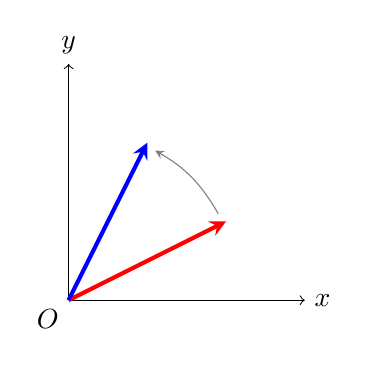
\begin{tikzpicture}
\draw[->] (0,0)--(3,0) node[right]{$x$};
\draw[->] (0,0)--(0,3) node[above]{$y$};
\draw[red,line width=1.5,-stealth] (0,0)--(2,1);
\draw[blue,line width=1.5,-stealth] (0,0)--(1,2);
\draw[gray,-stealth] (1.9,1.1) to [out=120,in=-30](1.1,1.9);
\node[below left]{$O$}; 
\end{tikzpicture}
\begin{tikzpicture}
\draw[gray,->] (0,0)--(3,0) node[right]{$x$};
\draw[gray,->] (0,0)--(0,3) node[above](vecu){$y$};
\draw[->] (0,0)--(2.719, 1.268) node[right]{$x'$};
\draw[->] (0,0)--(-1.268, 2.719) node[above](vecv){$y'$};
\draw[Green,-stealth, line width=1.5] (0,0)--(2.5,0.5);
\node[below left]{$O$}; 
\pic[draw, ->, "$\theta$", angle eccentricity=1.5, angle radius=0.75cm] {angle = vecu--0--vecv};
\end{tikzpicture}\\
\caption{\textit{Left: case (a), active transformation, and right: case (b), passive transformation, for a 2D rotation.}}
\label{fig:rotatereflect}
\end{figure}

The construction of a rotational or reflectional matrix requires the representation of the new unit axes in the old coordinate system as suggested in Theorem \ref{thm:bijectivechincoord}, but with the extra condition that they are orthogonal to each other. Once they are found, they can be combined column by column to form the \index{Transition Matrix}\keywordhl{transition matrix}. For an anti-clockwise (positive) rotation like the one to the right side of the figure above, we have
\begin{subequations}
\label{eqn:2drotate}
\begin{empheq}[left={\empheqlbrace}]{alignat=1}
\hat{x}' &= (\cos \theta) \hat{x} + (\sin \theta) \hat{y} \\
\hat{y}' &= (-\sin \theta) \hat{x} + (\cos \theta) \hat{y}
\end{empheq}
\end{subequations}
The corresponding transition matrix is then
\begin{align}
P_\beta^S &= \begin{bmatrix}
[\hat{x}']_S|[\hat{y}']_S    
\end{bmatrix} \nonumber \\
&= \begin{bmatrix}
\cos \theta & -\sin \theta \\
\sin \theta & \cos \theta
\end{bmatrix}
\end{align}
where $S$ represents the standard basis, and $\beta$ indicates the rotated coordinates system. Alternatively,
\begin{align*}
P_S^\beta &= (P_\beta^S)^{-1} \\
&= (P_\beta^S)^T & \text{(Properties \ref{proper:orthoinvT})}\\
&= \begin{bmatrix}
\cos \theta & \sin \theta \\
-\sin \theta & \cos \theta
\end{bmatrix}
\end{align*}
These two matrices can be compared to the one we see in the last chapter when we study the real variant of diagonalization for complex eigenvalues. \par
If we have an orthogonal matrix $P$, and a vector $\vec{v}_0$ in the standard basis, then computing $\vec{v}_n = P\vec{v}_0$ in a forward direction can be viewed as directly applying the corresponding rotation or reflection on the vector $\vec{v}_0$ to produce $\vec{v}_n$ while staying in the same coordinate frame. This is the case (a) we have discussed above. For case (b), it is the exact opposite. Rotation or reflection of the coordinate system, where the concerned vector $\vec{v}_0$ is fixed physically, is achieved by solving $\vec{v}_0 = P\vec{v}_n$ in a backward manner, or equivalently $\vec{v}_n = P^{-1}\vec{v}_0 = P^T\vec{v}_0$. Taking transpose, it becomes $\vec{v}_n^T = \vec{v}_0^T P$. In such a situation, the vector is still the same one in a physical sense, but represented in the new coordinate system. Most situations belong to case (b), on which thereafter we will focus our discussion.
\par
However, as a reminder, these two cases are much related. For example, an anti-clockwise/positive rotation of a vector in case (a), can be viewed as a clockwise/negative rotation of the coordinate system in case (b), and vice versa. The two operations are only differed by a transpose. For successive rotations and reflections, the net transition matrix $P_f$ is produced by taking the product of individual rotational and reflectional matrices each by each. One common convention has the order from right to left, where $\vec{v}_n = (P_n^T\cdots P_3^TP_2^TP_1^T)\vec{v}_0$, and thus $P_f^T = P_n^T\cdots P_3^TP_2^TP_1^T$. Another equivalent option is to do it from left to right by applying a transpose, as in
$\vec{v}_n^T = \vec{v}_0^T(P_1P_2P_3\cdots P_n)$, $P_f = P_1P_2P_3\cdots P_n$.

\begin{exmp}
Find the net transition matrix, if a rotation about $y$-axis of $40$ degree in the positive direction is done first to produce an intermediate coordinate system $x', y', z'$, and then a reflection across the $x'y'$ plane is made to generate the final coordinate system $x'', y'', z''$ (so the new $z''$ axis is the negative of $z'$ axis).
\end{exmp}
\begin{solution}
The first transition matrix is
\begin{align*}
P_1
&= 
\begin{bmatrix}
\cos(40^\circ) & 0 & \sin(40^\circ) \\
0 & 1 & 0 \\
-\sin(40^\circ) & 0 & \cos(40^\circ)
\end{bmatrix}
\end{align*}
The readers should verify this. The second transition matrix is simply
\begin{align*}
P_2
&= 
\left[\begin{array}{@{\,}wc{10pt}wc{10pt}wc{10pt}@{\,}}
1 & 0 & 0 \\
0 & 1 & 0 \\
0 & 0 & -1
\end{array}\right]    
\end{align*}
So the net transition matrix is
\begin{align*}
P_f &= P_1P_2 \\
&= 
\begin{bmatrix}
\cos(40^\circ) & 0 & \sin(40^\circ) \\
0 & 1 & 0 \\
-\sin(40^\circ) & 0 & \cos(40^\circ)
\end{bmatrix}
\left[\begin{array}{@{\,}wc{10pt}wc{10pt}wc{10pt}@{\,}}
1 & 0 & 0 \\
0 & 1 & 0 \\
0 & 0 & -1
\end{array}\right] \\
&= 
\begin{bmatrix}
\cos(40^\circ) & 0 & -\sin(40^\circ) \\
0 & 1 & 0 \\
-\sin(40^\circ) & 0 & -\cos(40^\circ)
\end{bmatrix}
\end{align*}
\end{solution}
Short Exercise: What happens if we reverse the order of rotation/reflection?\footnote{The transition matrix becomes
\begin{align*}
\left[\begin{array}{@{\,}wc{8pt}wc{8pt}wc{8pt}@{\,}}
1 & 0 & 0 \\
0 & 1 & 0 \\
0 & 0 & -1
\end{array}\right]   
\begin{bmatrix}
\cos(40^\circ) & 0 & \sin(40^\circ) \\
0 & 1 & 0 \\
-\sin(40^\circ) & 0 & \cos(40^\circ)
\end{bmatrix}
&=
\begin{bmatrix}
\cos(40^\circ) & 0 & \sin(40^\circ) \\
0 & 1 & 0 \\
\sin(40^\circ) & 0 & -\cos(40^\circ)
\end{bmatrix} \\
&\neq 
\begin{bmatrix}
\cos(40^\circ) & 0 & -\sin(40^\circ) \\
0 & 1 & 0 \\
-\sin(40^\circ) & 0 & -\cos(40^\circ)
\end{bmatrix}
\end{align*}
In general, finite rotations/reflections are not commutative and the order matters.
}

\begin{exmp}
\label{ex:rotateyz}
For a vector $\vec{v}_0$ in the three-dimensional standard basis $S$, if the coordinate system undergoes a positive rotation about the straight line $x = 0, y = z$ by a degree of $\theta$, find its representation $\vec{v}_n$ in the new system $\beta$.
\end{exmp}
\begin{solution}
The common way to construct a transition matrix is to find the new axes in terms of the old coordinates. However, in this case, it is harder because the axis about which the rotation occurs is not along any of the main axes. Here, we can do another rotation 
\begin{align*}
P_1 = 
\begin{bmatrix}
1 & 0 & 0 \\
0 & \cos(\SI{45}{\degree}) & \sin(\SI{45}{\degree}) \\
0 & -\sin(\SI{45}{\degree}) & \cos(\SI{45}{\degree})
\end{bmatrix}
=
\left[\begin{array}{@{\,}wc{12pt}wc{12pt}wc{12pt}@{\,}}
1 & 0 & 0 \\
0 & \frac{1}{\sqrt{2}} & \frac{1}{\sqrt{2}} \\
0 & -\frac{1}{\sqrt{2}} & \frac{1}{\sqrt{2}}
\end{array}\right]
\end{align*}
about the $x$-axis first with a degree of $\SI{45}{\degree}$ clockwise so that the intermediate $z'$ axis is oriented along the desired line, while the $y'$ axis points in the $x = 0, y = -z$ direction relative to the original coordinate frame. Then we can apply the required rotation in the intermediate coordinate system about that $z'$ axis, which has a simple transition matrix representation of
\begin{align*}
P_2 =
\begin{bmatrix}
\cos \theta & -\sin \theta & 0 \\
\sin \theta & \cos \theta & 0 \\
0 & 0 & 1
\end{bmatrix}
\end{align*}
Finally, we undo the effect of the first rotation via multiplying by its inverse $P_1^{-1}$ which is equal to $P_1^T$ due to orthogonality (Properties \ref{proper:orthoinvT}). 
\begin{figure}[ht!]
\centering
\begin{tikzpicture}[x={(-0.4cm, -0.9cm)}, y={(1cm, 0cm)}, z={(0cm, 1cm)}]
\node[above left]{$O$}; 
\draw[thick,->] (0,0,0) -- (0,0,2) node[anchor=north west]{$z$};
\draw[thick,->] (0,0,0) -- (2,0,0) node[anchor=north east]{$x$};
\draw[thick,->] (0,0,0) -- (0,2,0) node[anchor=west]{$y$};
\draw[gray,dashed] (0,0,0) -- (0,2,2);
\node[above left] at (0,0,-5) {$O$}; 
\draw[thick,->] (0,0,-5) -- (0,1.414,1.414-5);
\draw[thick,->] (0,0,-5) -- (2,0,-5);
\draw[thick,->] (0,0,-5) -- (0,1.414,-1.414-5);
\draw[gray,dashed] (0,0,-5) -- (0,0,-5+2);
\draw[->] (0,0,-5+1) to[out=0,in=120] (0,1.414/2,1.414/2-5);
\node[above left] at (0,5,-5) {$O$}; 
\draw[thick,->] (0,5,-5) -- (0,1.414+5,1.414-5);
\draw[thick,->] (0,5,-5) -- (1.414,1+5,-1-5);
\draw[thick,->] (0,5,-5) -- (-1.414,1+5,-1-5);
\draw[gray,dashed] (0,5,-5) -- (2,5,-5);
\draw[->] (1,5,-5) to[out=240,in=210] (1.414/2,1/2+5,-1/2-5);
\node at (0,5,-6.5) {$\theta$};
\node[above left] at (0,5,0) {$O$}; 
\draw[thick,->] (0,5,0) -- (1.414,1+5,1) node[below]{$x'$};
\draw[thick,->] (0,5,0) -- (-1,0.707+1+5,-0.707+1) node[right]{$y'$};
\draw[thick,->] (0,5,0) -- (1,-0.707+1+5,0.707+1) node[above]{$z'$};
\draw[gray,dashed] (0,5,0) -- (0,5+2,2);
\draw[red,->] (0,0.75+5,1.35) to[out=240,in=210] (0,1.25+5,0.85);
\draw[red,thick,->] (0,3,0) -- (0,4,0) node[midway,above]{$P_f$};
\draw[blue,thick,->] (0,3,-5) -- (0,4,-5) node[midway,below]{$P_2$};
\draw[blue,thick,->] (0,1,-2) -- (0,1,-3) node[midway,left]{$P_1$};
\draw[blue,thick,->] (0,6,-3) -- (0,6,-2) node[midway,right]{$P_1^{-1}$};
\end{tikzpicture}
\caption{\textit{Flowchart for Example \ref{ex:rotateyz}.}}
\end{figure}
Hence the net transition matrix is
\begin{align*}
P_f = P_1 P_2 P_1^{-1} &= P_1 P_2 P_1^T \\
&= \left[\begin{array}{@{\,}wc{12pt}wc{12pt}wc{12pt}@{\,}}
1 & 0 & 0 \\
0 & \frac{1}{\sqrt{2}} & \frac{1}{\sqrt{2}} \\
0 & -\frac{1}{\sqrt{2}} & \frac{1}{\sqrt{2}}
\end{array}\right]
\begin{bmatrix}
\cos \theta & -\sin \theta & 0 \\
\sin \theta & \cos \theta & 0 \\
0 & 0 & 1
\end{bmatrix}
\left[\begin{array}{@{\,}wc{12pt}wc{12pt}wc{12pt}@{\;}}
1 & 0 & 0 \\
0 & \frac{1}{\sqrt{2}} & -\frac{1}{\sqrt{2}} \\
0 & \frac{1}{\sqrt{2}} & \frac{1}{\sqrt{2}}
\end{array}\right] \\
&= 
\begin{bmatrix}
\cos{\theta} & -\frac{\sin{\theta}}{\sqrt{2}} & \frac{\sin{\theta}}{\sqrt{2}} \\
\frac{\sin{\theta}}{\sqrt{2}} & \frac{(\cos{\theta}) + 1}{2} & \frac{-(\cos{\theta}) + 1}{2} \\
-\frac{\sin{\theta}}{\sqrt{2}} & \frac{-(\cos{\theta}) + 1}{2} & \frac{(\cos{\theta}) + 1}{2}
\end{bmatrix}
\end{align*}
For any vector $\vec{v}_0 = (x_0,y_0,z_0)^T$ expressed in the standard coordinate basis, the new coordinates after rotation are then
\begin{align*}
\vec{v}_0 &= P_f \vec{v}_n \\
\vec{v}_n &= (P_f)^T\vec{v}_0 \\
&=
\begin{bmatrix}
\cos{\theta} & \frac{\sin{\theta}}{\sqrt{2}} & -\frac{\sin{\theta}}{\sqrt{2}} \\
-\frac{\sin{\theta}}{\sqrt{2}} & \frac{(\cos{\theta}) + 1}{2} & \frac{-(\cos{\theta}) + 1}{2} \\
\frac{\sin{\theta}}{\sqrt{2}} & \frac{-(\cos{\theta}) + 1}{2} & \frac{(\cos{\theta}) + 1}{2}
\end{bmatrix}
\begin{bmatrix}
x_0 \\
y_0 \\
z_0
\end{bmatrix} \\
&=
\begin{bmatrix}
(\cos{\theta})x_0 + (\frac{\sin{\theta}}{\sqrt{2}})y_0 + (-\frac{\sin{\theta}}{\sqrt{2}})z_0 \\
(-\frac{\sin{\theta}}{\sqrt{2}})x_0 + (\frac{(\cos{\theta}) + 1}{2})y_0 + (\frac{-(\cos{\theta}) + 1}{2})z_0 \\
(\frac{\sin{\theta}}{\sqrt{2}})x_0 + (\frac{-(\cos{\theta}) + 1}{2})y_0 + (\frac{(\cos{\theta}) + 1}{2})z_0
\end{bmatrix}
\end{align*}
\end{solution}
Short Exercise: For the example above, if $(x_0, y_0, z_0)^T = (0,1,1)^T$ and $\theta = \frac{\pi}{6}$, find $\vec{v}_n = (x_n, y_n, z_n)^T$.\footnote{It is
\begin{align*}
\begin{bmatrix}
\cos{\frac{\pi}{6}} & \frac{\sin{\frac{\pi}{6}}}{\sqrt{2}} & -\frac{\sin{\frac{\pi}{6}}}{\sqrt{2}} \\
-\frac{\sin{\frac{\pi}{6}}}{\sqrt{2}} & \frac{(\cos{\frac{\pi}{6}}) + 1}{2} & \frac{-(\cos{\frac{\pi}{6}}) + 1}{2} \\
\frac{\sin\frac{\pi}{6}}{\sqrt{2}} & \frac{-(\cos{\frac{\pi}{6}}) + 1}{2} & \frac{(\cos{\frac{\pi}{6}}) + 1}{2}
\end{bmatrix}
\begin{bmatrix}
0 \\
1 \\
1
\end{bmatrix}
=
\begin{bmatrix}
(\frac{\sqrt{3}}{2})(0) + (\frac{1}{2\sqrt{2}})(1) + (-\frac{1}{2\sqrt{2}})(1) \\
(-\frac{1}{2\sqrt{2}})(0) + (\frac{\frac{1}{2} + 1}{2})(1) + (\frac{-\frac{1}{2} + 1}{2})(1) \\
(\frac{1}{2\sqrt{2}})(0) + (\frac{-\frac{1}{2} + 1}{2})(1) + (\frac{\frac{1}{2} + 1}{2})(1)
\end{bmatrix}
=
\begin{bmatrix}
0 \\
1 \\
1
\end{bmatrix}
\end{align*}
In fact, all vectors in the form of $s(0,1,1)^T$ where $s$ is any number will keep the same coordinates after transformation, no matter what the value $\theta$ takes, because the vector is oriented exactly along the rotational axis in question.}

\section{Orthogonal Diagonalization}
\label{section:orthogonaldiagreal}

\index{Orthogonal Diagonalization}\keywordhl{Orthogonal diagonalization} is a special case of diagonalization, in which the transformation matrix $P$ used to diagonalize the target matrix $A$ is an orthogonal matrix. Since from Section \ref{section:diagonalizeidea} we know that diagonalization boils down to asking if there exists a basis, represented by the columns of $P$, such that $D = P^{-1}AP$ is diagonal, orthogonal diagonalization is equivalent to demanding further that such a basis, comprised of the eigenvectors of $A$, is orthonormal, i.e.\ $P$ is an orthogonal matrix. We will discuss the case where $A$ is a real matrix first.
\begin{defn}[Orthogonal Diagonalization]
\label{defn:orthodiagonal}
Orthogonal diagonalization on a real $n \times n$ square matrix $A$ is to find an orthogonal matrix $P$ that consists of columns being the $n$ orthonormal $\mathbb{R}^n$ eigenvectors of $A$ (Definition \ref{defn:orthomatrix}) such that
\begin{align}
P^{-1}AP = P^TAP = D \label{eqn:orthodiagonalPAP} 
\end{align}
is a real diagonal matrix (Properties \ref{proper:diagonalize} and \ref{proper:orthoinvT}).
\end{defn}
Note that the requirements of eigenvectors being $\mathbb{R}^n$ and hence orthogonality defined by the real dot product implicitly constrain us to work over $\mathbb{R}$ and only real eigenvalues are allowed. Not all real square matrices can be orthogonally diagonalized because orthogonal diagonalization is a stronger version of ordinary diagonalization and the requirement is unsurprisingly stricter. However, it turns out that there is a really simple criterion: whether the matrix is symmetric.
\begin{thm}
\label{thm:symdiag}
A real square matrix $A$ can be orthogonally diagonalized if and only if $A$ is symmetric.
\end{thm}
As a corollary, all symmetric real matrices have only real eigenvalues. The "only if" part is very easy to show.\footnote{Note that if $A$ is orthogonally diagonalizable then $A = PDP^{-1} = PDP^T$. Then $A^T = (PDP^T)^T = PD^TP^T = PDP^T = A$ since the transpose of any diagonal matrix $D^T = D$ is equal to itself.} On the other hand, the "if" part is much more difficult to derive and requires us to build some intermediate results first, which will be done sequentially in the remainder of this section. Since the transformation matrix $P$ used to diagonalize a given matrix $A$ is formed from the eigenvectors of $A$ as pointed out by Properties \ref{proper:diagonalize}, for $P$ to be an orthogonal matrix, obviously we need to show that these eigenvectors are orthogonal to each other if $A$ is symmetric. To this end, we have the following observation.
\begin{proper}
\label{proper:symortho}
Any two eigenvectors of a real, symmetric matrix corresponding to two distinct eigenvalues are always orthogonal to each other.
\end{proper}
\begin{proof}
Denote the two eigenvectors as $\vec{v}^{(1)}$ and $\vec{v}^{(2)}$ which have two different eigenvalues $\lambda_1$ and $\lambda_2$. Then consider the quantity $\vec{v}^{(1)} \cdot (A\vec{v}^{(2)})$ where $A$ is the real, symmetric matrix. By Definition \ref{defn:eigen}, it is equal to $\vec{v}^{(1)} \cdot (\lambda_{2}\vec{v}^{(2)}) = \lambda_{2}(\vec{v}^{(1)} \cdot \vec{v}^{(2)})$. At the same time, using Properties \ref{proper:dotproper} too, we have
\begin{align*}
\vec{v}^{(1)}\cdot (A\vec{v}^{(2)}) &= (A^T\vec{v}^{(1)})\cdot \vec{v}^{(2)} \\
&= (A\vec{v}^{(1)})\cdot \vec{v}^{(2)} &\text{($A$ is symmetric)} \\
&= (\lambda_1\vec{v}^{(1)})\cdot \vec{v}^{(2)} = \lambda_1(\vec{v}^{(1)} \cdot \vec{v}^{(2)}) &\text{(Definition \ref{defn:eigen} again)}
\end{align*}
Therefore
\begin{align*}
\vec{v}^{(1)} \cdot (A\vec{v}^{(2)}) =  \lambda_1(\vec{v}^{(1)} \cdot \vec{v}^{(2)}) &= \lambda_{2}(\vec{v}^{(1)}\cdot \vec{v}^{(2)}) \\
(\lambda_{1}-\lambda_{2})(\vec{v}^{(1)} \cdot \vec{v}^{(2)}) &= 0
\end{align*}
Since the two eigenvalues are required to be distinct, $\lambda_{1} \neq \lambda_{2}$, and $\vec{v}^{(1)} \cdot \vec{v}^{(2)}$ must be $0$. By Properties \ref{proper:dotorth}, the two eigenvectors $\vec{v}^{(1)}$ and $\vec{v}^{(2)}$ are orthogonal to each other.
\end{proof}
Even when there are multiple eigenvectors (a geometric multiplicity/an eigenspace of dimension $\geq 2$) associated with the same eigenvalue, we can mediate the problem by using the Gram-Schmidt Orthogonalization procedure introduced in Section \ref{section:GSortho} to produce an orthonormal basis to that eigenspace. Since all vectors in the eigenspace are subjected to the same eigenvalue, the choice of new eigenvectors will not disrupt the diagonalization process. So, with these, we have solved the "orthogonal" part of "orthogonal diagonalization", and the remaining half of the problem is to justify why symmetric matrices are always "diagonalizable", i.e.\ the geometric multiplicities of all their eigenvalues are equal to the corresponding algebraic multiplicities as suggested by Properties \ref{proper:diagonalize}\footnote{The another condition requires the characteristic polynomial to split over $\mathbb{R}$, but it is immediately satisfied due to the previous corollary to Theorem \ref{thm:symdiag} which points out that the eigenvalues of any symmetric matrix are always real (with Definition \ref{defn:charactereqn}).}, or in other words, there is no \textit{"deficient"} eigenvalue.
\begin{proper}
\label{proper:symnodefic}
The geometric multiplicity of any distinct eigenvalue of a real symmetric matrix is always strictly equal to its algebraic multiplicity.
\end{proper}
\begin{proof}
Let $A$ be some $n \times n$ real symmetric matrix. Denote the geometric multiplicity of any distinct eigenvalue $\lambda_{J_i}$ of $A$ by $n_{J_i}$ and its algebraic multiplicity by $k_{J_i}$. We will assume that $n_{J_i} < k_{J_i}$ and derive a contradiction. The geometric multiplicity of $n_{J_i}$ implies that there can be $n_{J_i}$ orthonormal (see the discussion above) eigenvectors $\smash{\vec{v}^{(1)}_{\lambda_{J_i}}}, \smash{\vec{v}^{(2)}_{\lambda_{J_i}}}, \ldots, \smash{\vec{v}^{(n_{J_i})}_{\lambda_{J_i}}} \in \mathbb{R}^n$ corresponding to $\lambda_{J_i}$ in the eigenspace $\mathcal{E}_{J_i}$. By part (c) of Properties \ref{proper:linindspanbasisnewver}, we can complete a basis $\mathcal{E}_{J_i} \oplus (\mathcal{E}_{J_i})^C$ for $\mathbb{R}^n$ by filling them with some other orthonormal $n-n_{J_i}$ vectors. Let $P$ be the orthogonal coordinate matrix that represents this basis in its columns, such that
\begin{align*}
P = \begin{bmatrix}
\vec{v}^{(1)}_{\lambda_{J_i}} | \vec{v}^{(2)}_{\lambda_{J_i}} | \cdots | \vec{v}^{(n_{J_i})}_{\lambda_{J_i}} | \text{other vectors used to fill the basis for $\mathbb{R}^n$}
\end{bmatrix}
\end{align*}
similar to the derivation of Theorem \ref{thm:geolessalgebra}. With the same logic, we can apply a change of coordinates for $A$ with $P$, such that
\begin{align*}
A' &= P^{-1}AP \\
&= \begin{bmatrix}
\lambda_{J_i} I_{n_{J_i}} & *_{n_{J_i}\times(n-n_{J_i})} \\
[\textbf{0}]_{(n-n_{J_i})\times n_{J_i}} & *_{(n-n_{J_i})\times(n-n_{J_i})}
\end{bmatrix}
\end{align*}
However, this time, as $P$ has been declared to be an orthogonal matrix, $A' = P^{-1}AP = P^TAP$ (Properties \ref{proper:orthoinvT}) can be easily shown to be symmetric like $A$ as well.\footnote{$(P^TAP)^T = P^TA^TP = P^TAP$.} Therefore, the upper-right block of $A'$ also has to be a zero submatrix (as the transpose of the zero submatrix to the lower left):
\begin{align*}
A' &=  
\begin{bmatrix}
\lambda_j I_{n_{J_i}} & [\textbf{0}]_{n_{J_i}\times(n-n_{J_i})} \\
[\textbf{0}]_{(n-n_{J_i})\times n_{J_i}} & *_{(n-n_{J_i})\times(n-n_{J_i})}
\end{bmatrix}
\end{align*}
which is now in the form of a matrix direct sum (see Definition \ref{defn:matdirectsum}). This shows that we can treat it as $A' = \lambda_j I_{n_{J_i}} \oplus A^C$ with respect to the $\mathcal{E}_{J_i} \oplus (\mathcal{E}_{J_i})^C$ vector direct sum basis following Definition \ref{defn:matdirectsum} where $A^C$ is an $(n-n_{J_i})\times(n-n_{J_i})$ matrix that makes up the bottom right asterisked block. From the perspective of a linear transformation, the restriction of $A'$ to $(\mathcal{E}_{J_i})^C$ is simply $A^C: (\mathcal{E}_{J_i})^C \to (\mathcal{E}_{J_i})^C$ which is a linear operator by itself. Now if the algebraic multiplicity of $\lambda_{J_i}$ is $k_{J_i}$, then $A$ will have a characteristic polynomial of 
\begin{align*}
p_A(\lambda) = (\lambda_{J_i}-\lambda)^{k_{J_i}} p^-(\lambda)    
\end{align*} where $p^-(\lambda)$ is some other polynomial. By Properties \ref{proper:similarinvariant}, $A'$ will also have this same characteristic polynomial $p_{A'}(\lambda) = (\lambda_{J_i}-\lambda)^{k_{J_i}} p^-(\lambda)$. At the same time, from the structure of $A'$ derived above, we know that 
\begin{align*}
p_{A'}(\lambda) = (\lambda_{J_i}-\lambda)^{n_{J_i}} p^C(\lambda)    
\end{align*} by repeated cofactor expansions along the first $n_{J_i}$ columns, with $p^C(\lambda)$ denoting the characteristic polynomial for $A^C$. Thus comparing the two expressions we know that 
\begin{align*}
p^C(\lambda) = (\lambda_j-\lambda)^{k_{J_i} - n_{J_i}}p^-(\lambda)    
\end{align*} Since we assume $n_{J_i} < k_{J_i}$, we know that $k_{J_i} - n_{J_i} \geq 1$, and $p^C(\lambda)$ will then contain some $(\lambda_j-\lambda)$ factor. Hence $A^C$, as a square matrix in its own right, must have an eigenvector $\smash{\vec{v}^{(n_{J_i}+1)}_{\lambda_{J_i}}}$ in the $(\mathcal{E}_{J_i})^C$ subspace corresponding to $\lambda_{J_i}$ since its geometric multiplicity in $A^C$ must be at least $1$. This $\smash{\vec{v}^{(n_{J_i}+1)}_{\lambda_{J_i}}}$ is also an eigenvector of the entire matrix $A$ and will be linearly independent of $\smash{\vec{v}^{(1)}_{\lambda_{J_i}}}, \smash{\vec{v}^{(2)}_{\lambda_{J_i}}}, \ldots, \smash{\vec{v}^{(n_{J_i})}_{\lambda_{J_i}}}$ because $\mathcal{E}_{J_i} \oplus (\mathcal{E}_{J_i})^C$ is a direct sum (Definition \ref{defn:directsum} this time). Therefore, this shows that the geometric multiplicity of $\lambda_{J_i}$ in $A$ is actually $n_{J_i}+1$ which contradicts our hypothesis that it is $n_{J_i}$, whenever $n_{J_i} < k_{J_i}$. (We can also inductively use this argument until the geometric multiplicity adds up to $k_{J_i}$.) Hence the only reasonable conclusion is $n_{J_i} = k_{J_i}$. 
\end{proof}
\par
Properties \ref{proper:symortho} and \ref{proper:symnodefic} together imply the "if" part of Theorem \ref{thm:symdiag} and the proof is completed. Recall that the essence of orthogonal diagonalization is to search for an orthonormal basis such that the linear operator or square matrix is diagonal with respect to it. These orthonormal basis vectors are at the same time the eigenvectors of the symmetric matrix following Properties \ref{proper:diagonalize}. Hence as a corollary,
\begin{proper}
\label{proper:orthobasissym}
A real $n \times n$ matrix has $n$ linearly independent eigenvectors that form an orthonormal basis for $\mathbb{R}^n$ if and only if it is symmetric if and only if it is orthogonally diagonalizable.
\end{proper}

\begin{exmp}
\label{exmp:orthodiag}
Carry out orthogonal diagonalization on the matrix
\begin{align*}
A =
\begin{bmatrix}
1 & 0 & 0 \\
0 & 2 & 1 \\
0 & 1 & 2
\end{bmatrix}
\end{align*}
\end{exmp}
\begin{solution}
First, we observe that $A$ is real and symmetric, and can be orthogonally diagonalized according to Theorem \ref{thm:symdiag}. It can be found that the eigenvectors, after normalization, are
\begin{align*}
&\vec{v}_\lambda = 
\left[
\begin{array}{wc{8pt}}
1 \\
0 \\
0
\end{array}\right] \text{ and }
\left[\begin{array}{wc{8pt}}
0 \\
-\frac{1}{\sqrt{2}} \\
\frac{1}{\sqrt{2}}
\end{array}\right]
& \text{for } \lambda = 1 \\
&\vec{v}_\lambda = 
\left[\begin{array}{wc{8pt}}
0 \\
\frac{1}{\sqrt{2}} \\
\frac{1}{\sqrt{2}}
\end{array}\right]
& \text{for } \lambda = 3
\end{align*}
Hence we can construct
\begin{align*}
P =
\left[\begin{array}{@{}wc{12pt}wc{12pt}wc{12pt}@{\,}}
1 & 0 & 0 \\
0 & -\frac{1}{\sqrt{2}} & \frac{1}{\sqrt{2}} \\
0 & \frac{1}{\sqrt{2}} & \frac{1}{\sqrt{2}}
\end{array}\right]
\end{align*}
So that
\begin{align*}
P^TAP &=
\left[\begin{array}{@{}wc{12pt}wc{12pt}wc{12pt}@{\,}}
1 & 0 & 0 \\
0 & -\frac{1}{\sqrt{2}} & \frac{1}{\sqrt{2}} \\
0 & \frac{1}{\sqrt{2}} & \frac{1}{\sqrt{2}}
\end{array}\right]^T
\begin{bmatrix}
1 & 0 & 0 \\
0 & 2 & 1 \\
0 & 1 & 2
\end{bmatrix}
\left[\begin{array}{@{}wc{12pt}wc{12pt}wc{12pt}@{\,}}
1 & 0 & 0 \\
0 & -\frac{1}{\sqrt{2}} & \frac{1}{\sqrt{2}} \\
0 & \frac{1}{\sqrt{2}} & \frac{1}{\sqrt{2}}
\end{array}\right] \\
&= 
\begin{bmatrix}
1 & 0 & 0\\
0 & 1 & 0\\
0 & 0 & 3 
\end{bmatrix} = D
\end{align*}
\end{solution}
Short Exercise: Confirm that $P$ is orthogonal.\footnote{It is simply checking
\begin{align*}
\begin{bmatrix}
1 & 0 & 0 \\
0 & -\frac{1}{\sqrt{2}} & \frac{1}{\sqrt{2}} \\
0 & \frac{1}{\sqrt{2}} & \frac{1}{\sqrt{2}}
\end{bmatrix}^T
\begin{bmatrix}
1 & 0 & 0 \\
0 & -\frac{1}{\sqrt{2}} & \frac{1}{\sqrt{2}} \\
0 & \frac{1}{\sqrt{2}} & \frac{1}{\sqrt{2}}
\end{bmatrix} = 
\begin{bmatrix}
1 & 0 & 0 \\
0 & 1 & 0 \\
0 & 0 & 1
\end{bmatrix}
\end{align*}
}

\subsubsection{Remark} From Properties \ref{proper:endomorph}, we know that orthogonal diagonalization $D = P^{-1}AP = P^TAP$ is simply a special case of coordinate transformation for a square matrix, where $P$ is now orthogonal and only pure rotations/reflections are involved (Theorem \ref{thm:orthodet}).

\section{Orthogonal Projections and Spectral Theorem}

\subsection{Projections onto a Subspace}

Another important concept that also involves orthogonality is \textit{orthogonal projections}. Back in Section \ref{section:proj} we have defined the projection of a vector $\vec{v}$ onto another vector $\vec{u}$, which is implicitly an orthogonal projection since the orthogonal component of $\vec{v}$ normal to $\vec{u}$ is removed while the parallel component of $\vec{v}$ along $\vec{u}$ is retained, i.e.\ $\vec{v} = \overrightarrow{\text{proj}}_u v + (\vec{v} - \overrightarrow{\text{proj}}_u v)$ and $\vec{u} \cdot (\vec{v} - \overrightarrow{\text{proj}}_u v) = 0$. Here we can treat $\vec{u}$ as the one-dimensional subspace generated by itself, and the projection of any vector $\vec{v}$ onto $\vec{u}$ is an operation to project the vector onto this subspace of $\text{span}(\{\vec{u}\})$. However, before digging deep into orthogonal projections, we have to first generalize the notion of projections involving multi-dimensional subspaces. Given two subspaces $\mathcal{W}_1$ and $\mathcal{W}_2$ of a vector space $\mathcal{V}$ which forms a direct sum $\mathcal{W}_1 \oplus \mathcal{W}_2 = \mathcal{V}$, the \textit{projection of a vector onto $\mathcal{W}_1$ along $\mathcal{W}_2$} is a linear operator $T:\mathcal{V} \to \mathcal{V}$ such that for any $\vec{v} = \vec{w}_1 + \vec{w}_2$\footnote{This decomposition of $\vec{v}$ into $\vec{w}_1$ and $\vec{w}_2$ is unique as $\mathcal{W}_1 \oplus \mathcal{W}_2$ is required to be a direct sum. (see Section \ref{section:directsum})} where $\vec{w}_1 \in \mathcal{W}_1$ and $\vec{w}_2 \in \mathcal{W}_2$, $T(\vec{v}) = \vec{w}_1$, so that only the $\mathcal{W}_1$ component is kept (projected onto) while the $\mathcal{W}_2$ component is discarded. Clearly, $\mathcal{R}(T) = \mathcal{W}_1$ and $\mathcal{N}(T) = \mathcal{W}_2$ is the range and kernel of $T$, and $\mathcal{R}(T) \oplus \mathcal{N}(T) = \mathcal{V}$. Here we give another equivalent definition of a projection.
\begin{proper}[Projection]
\label{proper:matrixproj}
A linear operator $T: \mathcal{V} \to \mathcal{V}$ is a projection if and only if $T^2 = T$.
\end{proper}
\begin{proof}
If $T^2 = T$, then for any $\vec{v} \in \mathcal{V}$, we have $T^2(\vec{v}) = T(T(\vec{v})) = T(\vec{v})$, therefore for any vector $T(\vec{v}) = \vec{w}_1 \in \mathcal{W}_1 = \mathcal{R}(T)$ in the range of $T$, $T(\vec{w}_1) = \vec{w}_1$, and the $\mathcal{W}_1$ component remains unchanged. Now, we demand $\mathcal{W}_2$ such that we can write $\vec{v} = \vec{w}_1 + (\vec{v} - \vec{w}_1) = \vec{w}_1 + \vec{w}_2$ for any $\vec{v} \in \mathcal{V}$, where $\vec{v} - \vec{w}_1 = \vec{w}_2 \in \mathcal{W}_2$ and $\mathcal{W}_1 \oplus \mathcal{W}_2 = \mathcal{V}$\footnote{$\mathcal{W}_2$ can be shown to be a subspace and is linearly independent of $\mathcal{W}_1$. The actual projection matrix $T$ is not only determined by $\mathcal{W}_1$ but also $\mathcal{W}_2$, since the choice of $\mathcal{W}_2$ will dictate $\vec{v} - \vec{w}_1 \in \mathcal{W}_2$ and hence $\vec{w}_1$ too.}. Applying $T$ on both sides gives 
\begin{align*}
T(\vec{v}) &= T(\vec{w}_1 + \vec{v} - \vec{w}_1) \\
T(\vec{v}) &= T(\vec{w}_1) + T(\vec{v} - \vec{w}_1) & \text{(Linearity from Definition \ref{defn:lintrans})}\\
\vec{w}_1 &= \vec{w}_1 + T(\vec{v} - \vec{w}_1) \\
\implies T(\vec{v} - \vec{w}_1) &= \textbf{0}
\end{align*}
So $T(\vec{v} - \vec{w}_1) = T(\vec{w}_2) = \textbf{0}$ for any $\vec{v} \in \mathcal{V}$ and $\vec{w}_2 \in \mathcal{W}_2$ as well. This shows that $\mathcal{W}_2 = \mathcal{N}(T)$ is the kernel of $T$ and any $\mathcal{W}_2$ component is annihilated. The "only if" part is simpler: given the effect of projection $T$ as defined in the beginning, for any arbitrary $\vec{v}$, $T^2(\vec{v}) = T(T(\vec{v})) = T(\vec{w}_1) = \vec{w}_1 = T(\vec{v})$, so by Properties \ref{proper:sametrans} it must be that $T^2 = T$.
\end{proof}
A linear operator/matrix $T$ satisfying the condition $T^2 = T$ is known as \index{Idempotent}\keywordhl{idempotent}, and we have $T^n = T$ for any positive integer $n$.\footnote{For $n \geq 2$, $T^n = (T^2) (T^{n-2}) = (T) (T^{n-2}) = T^{n-1}$ which can be recursively used.} So in other words, a linear operator is a projection if and only if it is idempotent.

\begin{exmp}
\label{exmp:xyproj}
Show that the linear operator $T$ which has a matrix representation of
\begin{align*}
[T] =
\begin{bmatrix}
0 & 1 \\
0 & 1 
\end{bmatrix}
\end{align*}
is a projection. Onto/along which subspace this projection is? 
\end{exmp}
\begin{solution}
By Properties \ref{proper:matrixproj}, we have to check if $[T]^2 = [T]$. A simple calculation yields
\begin{align*}
[T]^2 &=
\begin{bmatrix}
0 & 1 \\
0 & 1 
\end{bmatrix}
\begin{bmatrix}
0 & 1 \\
0 & 1 
\end{bmatrix} \\
&= 
\begin{bmatrix}
(0)(0) + (1)(0) & (0)(1) + (1)(1) \\
(0)(0) + (1)(0) & (0)(1) + (1)(1)
\end{bmatrix} \\
&= 
\begin{bmatrix}
0 & 1 \\
0 & 1 
\end{bmatrix} = [T]
\end{align*}
So it is indeed a projection. The subspace onto which the linear operator projects, is simply equal to its range, or equivalently the column space of $[T]$, which can be immediately identified as $\text{span}(\{(1,1)^T\})$, that is, the straight line $y=x$. Similarly, the projection is along its kernel/null space, which is also easily seen to be $\text{span}(\{(1,0)^T\})$, the $x$-axis.\par
\end{solution}

\begin{figure}[h!]
    \centering
    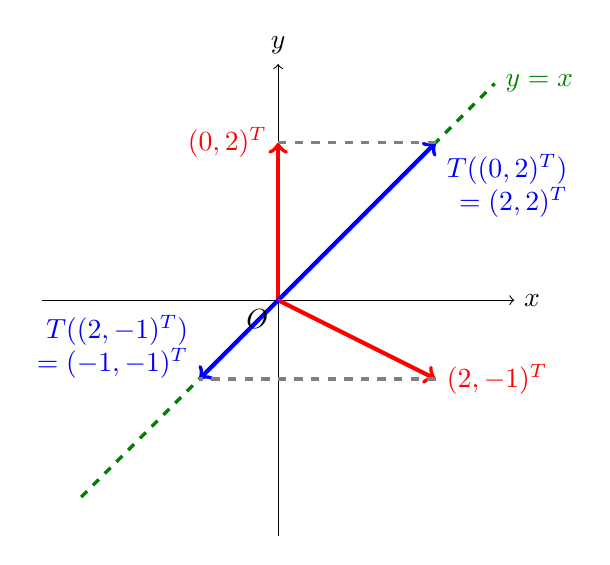
\begin{tikzpicture}
    \draw[->] (-3,0)--(3,0) node[right]{$x$};
    \draw[->] (0,-3)--(0,3) node[above]{$y$};
    \draw[dashed, Green, line width=1.2] (-2.5,-2.5) -- (2.75,2.75) node[right]{$y=x$};
    \draw[->, red, line width=1.5] (0,0) -- (0,2) node[left]{$(0,2)^T$};
    \draw[->, blue, line width=1.5] (0,0) -- (2,2) node[below right, align=right]{$T((0,2)^T)$\\ $= (2,2)^T$};
    \draw[->, red, line width=1.5] (0,0) -- (2,-1) node[right]{$(2,-1)^T$};
    \draw[->, blue, line width=1.5] (0,0) -- (-1,-1) node[above left, yshift=-4, align=right]{$T((2,-1)^T)$ \\ $= (-1,-1)^T$};
    \draw[dashed, gray, line width=1.2] (0,2) -- (2,2);
    \draw[dashed, gray, line width=1.2] (2,-1) -- (-1,-1);
    \node[below left]{$O$}; 
    \end{tikzpicture}
    \caption{\textit{Effects of projections (red to blue) in Example \ref{exmp:xyproj}.}}
\end{figure}

\subsection{Orthogonal Projections}
\label{subsection:orthoproj}

After knowing how projections onto a subspace look like, we can now properly generalize the \index{Orthogonal Projection}\keywordhl{orthogonal projection} (not to be confused with an orthogonal matrix) of a vector onto another vector, to a (possibly multi-dimensional) subspace. For a projection onto a subspace $\mathcal{W}_1$ along another subspace $\mathcal{W}_2$ to be an orthogonal projection, these two subspaces have to be the orthogonal complement to each other, such that for any $\vec{v} = \vec{w}_1 + \vec{w}_2$, $\vec{w}_1 \in \mathcal{W}_1$ and $\vec{w}_2 \in \mathcal{W}_2$, $\vec{w}_1$ and $\vec{w}_2$ are orthogonal (i.e.\ $\vec{w}_1 \cdot \vec{w}_2 = 0$, $\mathcal{W}_1^\perp = \mathcal{W}_2$ and $\mathcal{W}_2^\perp = \mathcal{W}_1$), and $T(\vec{v}) = \vec{w}_1$ means that the orthogonal component $\vec{w}_2 \in \mathcal{W}_2$ normal to $\mathcal{W}_1$ is removed. As there is only one orthogonal complement for any (finite-dimensional) subspace, the range $\mathcal{R}(T) = \mathcal{W}_1$ uniquely determines $\mathcal{N}(T) = \mathcal{W}_2$ and hence $T$, where $\mathcal{R}(T)^\perp = \mathcal{N}(T)$ and $\mathcal{N}(T)^\perp = \mathcal{R}(T)$ now. An equivalent condition of an orthogonal projection is that $[T] = [T]^T$ is symmetric given we are working over $\mathbb{R}$.\footnote{Some may wonder why in Properties \ref{proper:matrixproj} we use $T$ directly but here we circumvent by employing the matrix representation $[T]$ instead. It is because we haven't defined the "transpose" or "symmetric" equivalent for a linear operator, which will be introduced as the \textit{adjoint} in Chapter \ref{chap:innerchap}.}
\begin{proper}[Orthogonal Projection]
\label{proper:orthogonalproj}
A \textit{real}, \textit{finite-dimensional} linear projection operator $T: \mathcal{V} \to \mathcal{V}$ is an orthogonal projection (with respect to the usual real dot product) if and only if $[T] = [T]^T$ in terms of its matrix representation.  
\end{proper}
\begin{proof}
The "if" part: We need to show that $[T] = [T]^T$ implies $\mathcal{R}(T)^\perp = \mathcal{N}(T)$ (and $\mathcal{N}(T)^\perp = \mathcal{R}(T)$)\footnote{This two are equivalent as $\mathcal{V}$ is finite-dimensional.}. Let $\vec{w}_1 \in \mathcal{R}(T)$ and $\vec{w}_2 \in \mathcal{N}(T)$, then 
\begin{align*}
\vec{w}_1 \cdot \vec{w}_2 &= ([T]\vec{w}_1) \cdot \vec{w}_2 & \text{($T(\vec{w}_1) = \vec{w}_1$ by the definition of a projection)} \\
&= ([T]^T\vec{w}_1) \cdot \vec{w}_2 \\
&= \vec{w}_1 \cdot ([T]\vec{w}_2) & \text{(Properties \ref{proper:dotproper})} \\
&= \vec{w}_1 \cdot \textbf{0} = 0 & \text{($T(\vec{w}_2) = \textbf{0}$ by the definition of a projection)}
\end{align*}
So any $\vec{w}_2 \in \mathcal{N}(T)$ will be orthogonal to all $\vec{w}_1 \in \mathcal{R}(T)$ and $\mathcal{N}(T) \subseteq \mathcal{R}(T)^\perp$. Now let $\vec{w}_3 \in \mathcal{R}(T)^\perp$ and we want to show $\vec{w}_3 \in \mathcal{N}(T)$, i.e.\ $T(\vec{w}_3) = \textbf{0}$, such that $\mathcal{R}(T)^\perp \subseteq \mathcal{N}(T)$ and thus $\mathcal{R}(T)^\perp = \mathcal{N}(T)$. Consider $\vec{w}_3 \cdot T^2(\vec{w}_3)$ where $T^2(\vec{w}_3) \in \mathcal{R}(T)$ since $T^2 = T$ represents the action of projection (Properties \ref{proper:matrixproj}), and therefore $\vec{w}_3 \cdot T^2(\vec{w}_3) = 0$ as $\vec{w}_3 \in \mathcal{R}(T)^\perp$, but also
\begin{align*}
\vec{w}_3 \cdot T^2(\vec{w}_3) = \vec{w}_3 \cdot ([T]^2\vec{w}_3) &= \vec{w}_3 \cdot ([T]^T[T]\vec{w}_3) & \text{(By assumption)} \\
&= ([T]\vec{w}_3) \cdot ([T]\vec{w}_3) & \text{(Properties \ref{proper:dotproper})} \\
&= \norm{[T]\vec{w}_3}^2 = \norm{T(\vec{w}_3)}^2 
\end{align*}
Since this quantity is shown to be zero, $\norm{T(\vec{w}_3)} = 0$ and $T(\vec{w}_3) = \textbf{0}$ (see the remark below Properties \ref{proper:lengthdot}), and we are done.
\\
The "only if" part: Let $T$ be an orthogonal projection, $\vec{u} = \vec{w}_1^{(1)} + \vec{w}_2^{(1)}$ and $\vec{v} = \vec{w}_1^{(2)} + \vec{w}_2^{(2)}$ where $\vec{w}_1^{(1)}, \vec{w}_1^{(2)} \in \mathcal{W}_1 = \mathcal{R}(T)$ and $\vec{w}_2^{(1)}, \vec{w}_2^{(2)} \in \mathcal{W}_2 = \mathcal{N}(T)$. Consider 
\begin{align*}
\vec{u} \cdot T(\vec{v}) = (\vec{w}_1^{(1)} + \vec{w}_2^{(1)}) \cdot (\vec{w}_1^{(2)}) &= \vec{w}_1^{(1)} \cdot \vec{w}_1^{(2)} + \vec{w}_2^{(1)} \cdot \vec{w}_1^{(2)} \\
&= \vec{w}_1^{(1)} \cdot \vec{w}_1^{(2)}
\end{align*}
where $\vec{w}_2^{(1)} \cdot \vec{w}_1^{(2)} = 0$ because $\mathcal{N}(T) = \mathcal{R}(T)^\perp$. Similarly we have $[T]\vec{u} \cdot \vec{v} = T(\vec{u}) \cdot \vec{v} = \vec{w}_1^{(1)} \cdot \vec{w}_1^{(2)} + \vec{w}_1^{(1)} \cdot \vec{w}_2^{(2)} = \vec{w}_1^{(1)} \cdot \vec{w}_1^{(2)} = \vec{u} \cdot T(\vec{v})$. At the same time
\begin{align*}
\vec{u} \cdot T(\vec{v}) &= \vec{u} \cdot ([T]\vec{v}) \\
&= ([T]^T\vec{u}) \cdot \vec{v} & \text{(Properties \ref{proper:dotproper})}
\end{align*}
This shows that $([T]\vec{u}) \cdot \vec{v} = ([T]^T\vec{u}) \cdot \vec{v}$ for any $\vec{u}, \vec{v} \in \mathcal{V}$. Particularly, since this equality holds for any $\vec{v} \in \mathcal{V}$, it is always true that $[T]\vec{u} = [T]^T\vec{u}$, which further holds for any $\vec{u} \in \mathcal{V}$ and we conclude that $[T] = [T]^T$.
\end{proof}

\begin{exmp}
\label{exmp:xyproj2}
Example \ref{exmp:xyproj} has illustrated a projection in $\mathbb{R}^2$ onto the straight line $y = x$ along the $x$-axis. Continuing from this example, find the unique orthogonal projection onto the same line of $y = x$ correspondingly.
\end{exmp}
\begin{solution}
The matrix representation of $T$ is derived following Definition \ref{defn:matrixrepoflintrans}, during which the standard coordinates are used:
\begin{align*}
[T] =
\begin{bmatrix}
T(\hat{e}^{(1)})|T(\hat{e}^{(2)})
\end{bmatrix}
\end{align*}
Its columns are the outputs of applying the orthogonal projection on the standard unit vectors. Geometrically (see Figure \ref{fig:xyproj2} below), it can be easily deduced that $T(\hat{e}^{(1)}) = T(\hat{e}^{(2)}) = (\frac{1}{2}, \frac{1}{2})^T$, and hence
\begin{align*}
[T] =
\begin{bmatrix}
\frac{1}{2} & \frac{1}{2} \\
\frac{1}{2} & \frac{1}{2} 
\end{bmatrix}
\end{align*}
As a small example, given $\vec{v}=(1,-2)^T$, then the orthogonal projection of $\vec{v}$ onto the straight $y=x$ is computed as
\begin{align*}
T(\vec{v}) = [T](1,-2)^T = 
\begin{bmatrix}
\frac{1}{2} & \frac{1}{2} \\
\frac{1}{2} & \frac{1}{2}     
\end{bmatrix}
\begin{bmatrix}
1 \\
-2
\end{bmatrix}
=
\begin{bmatrix}
-\frac{1}{2} \\
-\frac{1}{2}
\end{bmatrix}
\end{align*}
\end{solution}
\begin{figure}[h!]
    \centering
    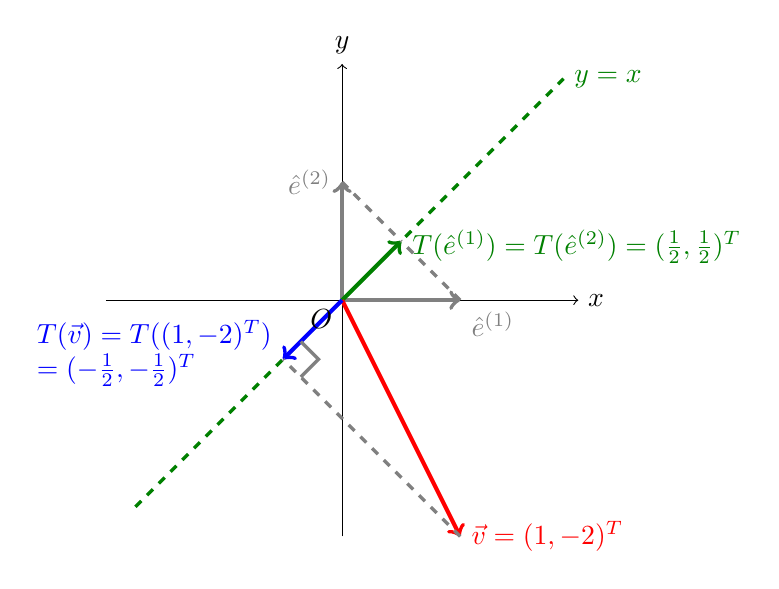
\begin{tikzpicture}[scale=1.5]
    \draw[->] (-2,0)--(2,0) node[right]{$x$};
    \draw[->] (0,-2)--(0,2) node[above]{$y$};
    \draw[dashed, Green, line width=1.2] (-1.75,-1.75) -- (1.875,1.875) node[right]{$y=x$};
    \draw[->, Gray, line width=1.5] (0,0) -- (1,0) node[below right]{$\hat{e}^{(1)}$};
    \draw[->, Gray, line width=1.5] (0,0) -- (0,1) node[left]{$\hat{e}^{(2)}$};
    \draw[->, Green, line width=1.5] (0,0) -- (0.5,0.5) node[yshift=-2, right]{$T(\hat{e}^{(1)}) = T(\hat{e}^{(2)}) = (\frac{1}{2}, \frac{1}{2})^T$};
    \draw[->, red, line width=1.5] (0,0) -- (1,-2) node[right]{$\vec{v} = (1,-2)^T$};
    \draw[->, blue, line width=1.5] (0,0) -- (-0.5,-0.5) node[left, yshift=2, align=left]{$T(\vec{v}) = T((1,-2)^T)$ \\ $= (-\frac{1}{2},-\frac{1}{2})^T$};
    \draw[dashed, gray, line width=1.2] (1,0) -- (0.5,0.5);
    \draw[dashed, gray, line width=1.2] (0,1) -- (0.5,0.5);
    \draw[dashed, gray, line width=1.2] (1,-2) -- (-0.5,-0.5);
    \draw[gray, line width=1.2] (-0.35,-0.35) -- (-0.2,-0.5) -- (-0.35,-0.65);
    \node[below left]{$O$}; 
    \end{tikzpicture}
    \caption{\textit{Illustration for Example \ref{exmp:xyproj2}.}}
    \label{fig:xyproj2}
\end{figure}

\begin{exmp}
\label{exmp:planeorthoproj}
Find the matrix for the orthogonal projection in $\mathbb{R}^3$ onto the subspace described by the plane $x + 2y - 4z = 0$.
\end{exmp}
\begin{solution}
In a higher-dimensional scenario, it is beneficial to derive an orthonormal basis for both the range $\mathcal{R}(T)$ and kernel $\mathcal{N}(T)$ of the orthogonal projection $T$ first, and work out the projection transformation in the coordinate system according to this basis. We can follow a similar approach as in Example \ref{exmp:vecgeohighdim}, and one possible basis for the plane is simply $\{(4,0,1)^T, (0,2,1)^T\}$. Subsequently, we can apply Gram-Schmidt orthogonalization (Definition \ref{defn:GSorth_norm}) to obtain an orthonormal basis for the plane. We leave it to the readers to check that it is $\{(\frac{4}{\sqrt{17}}, 0, \frac{1}{\sqrt{17}})^T, (-\frac{2}{\sqrt{357}}, \frac{17}{\sqrt{357}}, \frac{8}{\sqrt{357}})^T\}$. Motivated by Properties \ref{proper:orthodirectsum}, we will derive the third vector to complete an orthonormal basis for $\mathbb{R}^3$ and it will represent the kernel $\mathcal{N}(T) = \mathcal{R}(T)^\perp$ as the orthogonal complement to the plane. A quick way is to utilize cross product which yields $(\frac{4}{\sqrt{17}}, 0, \frac{1}{\sqrt{17}})^T \times (-\frac{2}{\sqrt{357}}, \frac{17}{\sqrt{357}}, \frac{8}{\sqrt{357}})^T = (-\frac{1}{\sqrt{21}}, -\frac{2}{\sqrt{21}}, \frac{4}{\sqrt{21}})^T$. The projection in this basis $\beta = \{(\frac{4}{\sqrt{17}}, 0, \frac{1}{\sqrt{17}})^T, (-\frac{2}{\sqrt{357}}, \frac{17}{\sqrt{357}}, \frac{8}{\sqrt{357}})^T, (-\frac{1}{\sqrt{21}}, -\frac{2}{\sqrt{21}}, \frac{4}{\sqrt{21}})^T\}$ will have a matrix representation of
\begin{align*}
[T]_\beta = 
\begin{bmatrix}
1 & 0 & 0 \\
0 & 1 & 0 \\
0 & 0 & 0
\end{bmatrix}
\end{align*}
as the first two basis vectors are in the range $\mathcal{R}(T)$ and will be projected into itself, while the last basis vector is in the kernel $\mathcal{N}(T)$ and hence annihilated. Now we can transform the projection matrix back into the standard basis system according to (\ref{eqn:endomorphcoordch}) of Properties \ref{proper:endomorph}, where
\begin{align*}
P_\beta^S = 
\begin{bmatrix}
\frac{4}{\sqrt{17}} & -\frac{2}{\sqrt{357}} & -\frac{1}{\sqrt{21}} \\
0 & \frac{17}{\sqrt{357}} & -\frac{2}{\sqrt{21}} \\
\frac{1}{\sqrt{17}} & \frac{8}{\sqrt{357}} & \frac{4}{\sqrt{21}}
\end{bmatrix}
\end{align*}
and
\begin{align*}
[T]_S &= (P_S^\beta)^{-1} [T]_\beta P_S^\beta \\
&= P_\beta^S [T]_\beta (P_\beta^S)^T \text{\quad (Properties \ref{proper:orthoinvT} for the orthogonal $P$ matrix)} \\
&=
\begin{bmatrix}
\frac{4}{\sqrt{17}} & -\frac{2}{\sqrt{357}} & -\frac{1}{\sqrt{21}} \\
0 & \frac{17}{\sqrt{357}} & -\frac{2}{\sqrt{21}} \\
\frac{1}{\sqrt{17}} & \frac{8}{\sqrt{357}} & \frac{4}{\sqrt{21}}
\end{bmatrix}
\begin{bmatrix}
1 & 0 & 0 \\
0 & 1 & 0 \\
0 & 0 & 0
\end{bmatrix}
\begin{bmatrix}
\frac{4}{\sqrt{17}} & -\frac{2}{\sqrt{357}} & -\frac{1}{\sqrt{21}} \\
0 & \frac{17}{\sqrt{357}} & -\frac{2}{\sqrt{21}} \\
\frac{1}{\sqrt{17}} & \frac{8}{\sqrt{357}} & \frac{4}{\sqrt{21}}
\end{bmatrix}^T \\
&=
\begin{bmatrix}
\frac{20}{21}&-\frac{2}{21}&\frac{4}{21}\\ 
-\frac{2}{21}&\frac{17}{21}&\frac{8}{21}\\ 
\frac{4}{21}&\frac{8}{21}&\frac{5}{21}
\end{bmatrix}
\end{align*}
To cross-check that $[T]_S$ indeed represents an orthogonal projection, it is obvious that $[T]_S$ is symmetric and the readers can verify that $[T]_S^2 = [T]_S$. Another cross-checking method is to pick a vector in the range [kernel], e.g. $\vec{v}_R = (6,1,2)^T$ and confirm that the projection $[T]_S\vec{v}_R = [T]_S(6,1,2)^T = (6,1,2)^T = \vec{v}_R$ leaves it unchanged [vanished].
\end{solution}
Now we can revisit the projection of a vector $\vec{v}$ onto another vector $\vec{u}$ as a special case of orthogonal projection in this section. In Definition \ref{proper:proj}, the projection acting on $\vec{v}$ is given as \begin{align*}
\overrightarrow{\text{proj}}_u v = \frac{\vec{v} \cdot \vec{u}}{\norm{\vec{u}}^2} \vec{u}    
\end{align*} which can be rewritten as
\begin{align*}
T(\vec{v}^T) &= \frac{1}{\norm{\textbf{u}}^2}(\textbf{v}^T\textbf{u})\textbf{u}^T \\
\implies T(\vec{v}) &= \frac{1}{\norm{\textbf{u}}^2}(\textbf{v}^T\textbf{u}\textbf{u}^T)^T \\
&= (\frac{1}{\norm{\textbf{u}}^2}\textbf{u}\textbf{u}^T)\textbf{v} \\
&= (\frac{\textbf{u}}{\norm{\textbf{u}}}(\frac{\textbf{u}}{\norm{\textbf{u}}})^T)\textbf{v} = [T]\textbf{v}
\end{align*}
where the orthogonal projection matrix is 
\begin{align}
[T] = \frac{\textbf{u}}{\norm{\textbf{u}}}(\frac{\textbf{u}}{\norm{\textbf{u}}})^T = \hat{\textbf{u}}\hat{\textbf{u}}^T    
\end{align} which is clearly symmetric and can be shown that $[T]^2 = [T]$.\footnote{$(\hat{\textbf{u}}\hat{\textbf{u}}^T)(\hat{\textbf{u}}\hat{\textbf{u}}^T) = \hat{\textbf{u}}(\hat{\textbf{u}}^T\hat{\textbf{u}})\hat{\textbf{u}}^T = \hat{\textbf{u}}(1)\hat{\textbf{u}}^T = \hat{\textbf{u}}\hat{\textbf{u}}^T$ as $\hat{\textbf{u}}$ is a unit vector and the dot product $\hat{\textbf{u}}^T\hat{\textbf{u}} = \vec{u}\cdot\vec{u} = \norm{\vec{u}}^2 = 1$ is its square length which simply equals $1$.} For an orthogonal projection $T$ in $\mathbb{R}^n$ onto some $r$-dimensional subspace, which becomes its range $\mathcal{R}(T)$ with an orthonormal basis $\{\vec{w}^{(1)}, \vec{w}^{(2)}, \ldots, \vec{w}^{(r)}\}$, complete this orthonormal basis for $\mathbb{R}^n$ by appending another orthonormal basis $\{\vec{w}^{(r+1)}, \ldots, \vec{w}^{(n)}\}$ of its kernel $\mathcal{N}(T) = \mathcal{R}(T)^\perp$ (possible due to Definition \ref{defn:GSorth_norm} and Properties \ref{proper:orthodirectsum}) just like Example \ref{exmp:planeorthoproj} above. By the same argument in that example, we know that
\begin{subequations}
\begin{align}
[T] &= 
\footnotesize
\begin{bmatrix}
\vec{w}^{(1)}|\cdots|\vec{w}^{(r)}|\vec{w}^{(r+1)}|\cdots|\vec{w}^{(n)}
\end{bmatrix}
\begin{bmatrix}
I_r & [\textbf{0}]_{r\times(n-r)} \\
[\textbf{0}]_{(n-r)\times r} & [\textbf{0}]_{(n-r)\times(n-r)} \\
\end{bmatrix}
\left[\begin{array}{c} 
\vec{w}^{(1)T} \\
\hline
\vdots \\
\hline
\vec{w}^{(r)T} \Tstrut \\
\hline
\vec{w}^{(r+1)T} \Tstrut\\
\hline 
\vdots \\
\hline
\vec{w}^{(n)T} \Tstrut
\end{array}\right] \\
&= \hat{\textbf{w}}^{(1)}\hat{\textbf{w}}^{(1)T} + \hat{\textbf{w}}^{(2)}\hat{\textbf{w}}^{(2)T} + \cdots + \hat{\textbf{w}}^{(r)}\hat{\textbf{w}}^{(r)T} \label{eqn:projrank1sum}
\end{align}
\end{subequations}
which generalizes the form of an orthogonal projection matrix above in the case of a multi-dimensional range. Furthermore, geometrically, the shortest distance of a point to a subspace is found by the orthogonal projection of that point onto the subspace.
\begin{proper}
\label{proper:shortestorthoproj}
The shortest distance of a subspace $\mathcal{W} \subset \mathcal{V}$ to some point $\vec{v} \in \mathcal{V}$ is achieved by $\vec{v} - T(\vec{v})$ where $T$ is the orthogonal projection operator onto $\mathcal{W}$.
\end{proper}
\begin{proof}
For any other point $\vec{w} \in \mathcal{W}$, we have
\begin{align*}
\norm{\vec{v} - \vec{w}}^2 &= \norm{(\vec{v} - T(\vec{v})) + (T(\vec{v}) - \vec{w})}^2 \\
&= \norm{\vec{v} - T(\vec{v})}^2 + \norm{T(\vec{v}) - \vec{w}}^2 + 2 (\vec{v} - T(\vec{v})) \cdot (T(\vec{v}) - \vec{w})
\end{align*}
Note that $\vec{v} - T(\vec{v}) \in \mathcal{N}(T) = \mathcal{R}(T)^\perp$ and $T(\vec{v}) - \vec{w} \in \mathcal{R}(T)$ as $T$ is a projection onto $\mathcal{W}$. Therefore, $(\vec{v} - T(\vec{v})) \cdot (T(\vec{v}) - \vec{w}) = 0$, and 
\begin{subequations}
\begin{align}
\norm{\vec{v} - \vec{w}}^2 &= \norm{\vec{v} - T(\vec{v})}^2 + \norm{T(\vec{v}) - \vec{w}}^2 > \norm{T(\vec{v}) - \vec{w}}^2 \label{eqn:shortestsubspacealta} \\
& > \norm{\vec{v} - T(\vec{v})}^2 \label{eqn:shortestsubspacealtb}
\end{align}
\end{subequations}
as $\vec{w} \neq T(\vec{v})$, $\norm{T(\vec{v}) - \vec{w}}^2 > 0$.
\end{proof}
\subsection{Spectral Theorem}
With orthonormal matrices and projections defined, we have come to the most important theorem in this chapter, the \index{Spectral Theorem}\keywordhl{Spectral Theorem}.
\begin{thm}[Spectral Theorem]
\label{thm:spectral}
For a linear operator $T: \mathcal{V} \to \mathcal{V}$ where $\mathcal{V}$ is a real, finite($n$)-dimensional vector space and the matrix representation of $T$ is symmetric, i.e.\ $[T]=[T]^T$, denote its eigenvalues by $\lambda_j$, $j = 1,2,\ldots,n$ (counting repeated ones). Assume there are $k$ distinct eigenvalues out of them. For every such a distinct eigenvalue, collect all the indices $j$ where $\lambda_j$ points to that same eigenvalue, let's say, $\lambda_{J_i}$, and group them into an index set $J_i$, $i = 1,2,\ldots,k$. Let the associated eigenspace be $\mathcal{E}_{J_i}$ for the $k$ sets of $J_i$ and denote the orthogonal projection onto $\mathcal{E}_{J_i}$ as $T_{J_i}$, then we have:
\begin{enumerate}[label=(\alph*)]
\item $\mathcal{V} = \mathcal{E}_{J_1} \oplus \mathcal{E}_{J_2} \oplus \cdots \oplus \mathcal{E}_{J_k} = \bigoplus_{i=1}^{k} \mathcal{E}_{J_i}$;
\item $(\bigoplus_{i \in \{I\}} \mathcal{E}_{J_i})^\perp = \bigoplus_{i \notin \{I\}} \mathcal{E}_{J_i}$ where $I$ is an index set containing some integers between $1$ and $k$;
\item $T_{J_i} T_{J_{i'}} = 
\begin{cases}
T_{J_i} & \text{if $i = i'$} \\
0 & \text{if $i \neq i'$}
\end{cases}$;
\item $I = T_{J_1} + T_{J_2} + \cdots + T_{J_k} = \sum_{i=1}^{k} T_{J_i}$; and
\item $T = \lambda_{J_1}T_{J_1} + \lambda_{J_2}T_{J_2} + \cdots + \lambda_{J_k}T_{J_k} = \sum_{i=1}^{k} \lambda_{J_i}T_{J_i}$.
\end{enumerate}
\end{thm}
\begin{proof}
\begin{enumerate}[label=(\alph*)]  
\item By Theorem \ref{thm:symdiag}, $[T]$ is (orthogonally) diagonalizable. The prior discussion in Section \ref{section:diagonalproper} has shown that
\begin{align*}
\bigoplus_{i=1}^{k} \mathcal{E}_{J_i} = \bigoplus_{j=1}^n \mathcal{E}_j = \mathcal{V} 
\end{align*}
where $\mathcal{E}_{J_i} = \bigoplus_{j \in J_i} \mathcal{E}_j$ is the direct sum of one-dimensional subspaces generated by each of the linearly independent eigenvector corresponding to the same eigenvalue $\lambda_{J_i}$.
\item This is a consequence of applying Properties \ref{proper:orthodirectsum} on (a) where $\bigoplus_{i \in \{I\}} \mathcal{E}_{J_i}$ and $\bigoplus_{i \notin \{I\}} \mathcal{E}_{J_i}$ are derived from the two mutually exclusive portions of the orthonormal basis for $\mathcal{V}$ that contains the $n$ orthonormal eigenvectors of the symmetric $[T]$, available due to the implication of Theorem \ref{proper:orthobasissym}.
\item $T_{J_i}^2 = T_{J_i}$ by the definition of a projection (Properties \ref{proper:matrixproj}). Also, we can express any $\vec{v} = \vec{v}_{J_1} + \vec{v}_{J_2} + \cdots + \vec{v}_{J_k}$ by (a) where $\vec{v}_{J_i} \in \mathcal{E}_{J_i}$. Then $T_{J_{i'}}(\vec{v}) = \vec{v}_{J_{i'}}$ due to the definition of an orthogonal projection and (b) where $\mathcal{E}_{J_{i'}}^\perp = \bigoplus_{i \neq i'} \mathcal{E}_{J_i}$. Using the same argument again means that $T_{J_i}(T_{J_i'}(\vec{v})) = T_{J_i}(\vec{v}_{J_{i'}}) = \textbf{0}$ if $i \neq i'$. Since this holds for any $\vec{v}$, $T_{J_i} T_{J_{i'}} = 0$.
\item Again for any $\vec{v}$ we can rewrite it as $\vec{v} = \vec{v}_{J_1} + \vec{v}_{J_2} + \cdots + \vec{v}_{J_k}$, $\vec{v}_{J_i} \in \mathcal{E}_{J_i}$. Since $T_{J_i}$ is an orthogonal projection onto $\mathcal{E}_{J_i}$, and also $\mathcal{E}_{J_{i}}^\perp = \bigoplus_{i \neq i'} \mathcal{E}_{J_i'} = \mathcal{N}(T_{J_i})$, we have $T_{J_i}(\vec{v}) = \vec{v}_{J_i}$. Thus $I(\vec{v}) = \vec{v} = \vec{v}_{J_1} + \vec{v}_{J_2} + \cdots + \vec{v}_{J_k} = T_{J_1}(\vec{v}) + T_{J_2}(\vec{v}) + \cdots + T_{J_k}(\vec{v}) = (T_{J_1} + T_{J_2} + \cdots + T_{J_k})(\vec{v})$ and it must be that $I = T_{J_1} + T_{J_2} + \cdots + T_{J_k}$ by Properties \ref{proper:sametrans}.
\item As usual, $\vec{v} = \vec{v}_{J_1} + \vec{v}_{J_2} + \cdots + \vec{v}_{J_k}$ and
\begin{align*}
T(\vec{v}) &= T(\vec{v}_{J_1}) + T\vec{v}_{J_2} + \cdots + T(\vec{v}_{J_k}) \\
&= \lambda_{J_1}\vec{v}_{J_1} + \lambda_{J_2}\vec{v}_{J_2} + \cdots + \lambda_{J_k}\vec{v}_{J_k} \quad \begin{aligned}
&\text{(Definition \ref{defn:eigen} for} \\
&\text{eigenvalues/eigenvectors)}
\end{aligned} \\
&= \lambda_{J_1}T_{J_1}(\vec{v}) + \lambda_{J_2}T_{J_2}(\vec{v}) + \cdots + \lambda_{J_k}T_{J_k}(\vec{v}) \text{\quad (Just as (d))} \\
&= (\lambda_{J_1}T_{J_1} + \lambda_{J_2}T_{J_2} + \cdots + \lambda_{J_k}T_{J_k})(\vec{v})
\end{align*}
and thus the desired relation follows, again by Properties \ref{proper:sametrans}.
\end{enumerate}
\end{proof}
The set of eigenvalues $\{\lambda_{J_i}\}$, $i = 1,2,\ldots,k$, is known as the \index{Spectrum}\keywordhl{spectrum} of $T$, hence comes the name of the theorem. The expression in (d) is called the \index{Resolution of the Identity}\keywordhl{resolution of the identity} induced by $T$, and that in (e) is referred to as the \index{Spectral Decomposition}\keywordhl{spectral decomposition} of $T$. The implications of these two parts of the Spectral Theorem are as follows: The resolution of the identity in (d) means that any vector $\vec{v}$ can be decomposed into components in the orthogonal coordinate system derived from the orthonormal eigenvectors of a symmetric $T$, where the corresponding coordinates are given by simply projecting it onto each of these eigenspaces; The spectral decomposition in (e) means that any symmetric linear operator $T$, when applied on a vector $\vec{v}$, can be treated as equivalent to first decomposing $\vec{v}$ into components in the orthogonal coordinate system as suggested by (d), and then rescaling each of these components according to the spectrum (eigenvalues), which represents the "intensity" of $T$ in the respective eigenspace. Since only projections and rescalings are involved, it implies that the symmetric $T$ constitutes no rotation. Finally, notice that an orthogonal projection is a special case of (e) where the spectrum consists of $1$ (range) and $0$ (kernel) only.\par
Short Exercise: Verify statements (d) and (e) in the Spectral Theorem for the symmetric matrix in Example \ref{exmp:orthodiag}.\footnote{We will just show (d) here and leave (e) to the readers. By Equation (\ref{eqn:projrank1sum}), R.H.S. of (d) reads
\begin{align*}
T_{J_1} + T_{J_2} &= (\textbf{v}_{J_1}^{(1)T}\textbf{v}_{J_1}^{(1)T} + \textbf{v}_{J_1}^{(2)T}\textbf{v}_{J_1}^{(2)T}) + \textbf{v}_{J_2}^{(1)T}\textbf{v}_{J_2}^{(1)T} \\
&= \begin{bmatrix}
1 \\
0 \\
0
\end{bmatrix}
\begin{bmatrix}
1 & 0 & 0
\end{bmatrix} + 
\begin{bmatrix}
0 \\
-\frac{1}{\sqrt{2}} \\
\frac{1}{\sqrt{2}}
\end{bmatrix}
\begin{bmatrix}
0 & -\frac{1}{\sqrt{2}} & \frac{1}{\sqrt{2}}
\end{bmatrix} +
\begin{bmatrix}
0 \\
\frac{1}{\sqrt{2}} \\
\frac{1}{\sqrt{2}}
\end{bmatrix}
\begin{bmatrix}
0 & \frac{1}{\sqrt{2}} & \frac{1}{\sqrt{2}}
\end{bmatrix} \\
&=
\begin{bmatrix}
1 & 0 & 0 \\
0 & 0 & 0 \\
0 & 0 & 0
\end{bmatrix}
+
\begin{bmatrix}
0 & 0 & 0 \\
0 & \frac{1}{2} & -\frac{1}{2} \\
0 & -\frac{1}{2} & \frac{1}{2}
\end{bmatrix}
+
\begin{bmatrix}
0 & 0 & 0 \\
0 & \frac{1}{2} & \frac{1}{2} \\
0 & \frac{1}{2} & \frac{1}{2}
\end{bmatrix}\
=
\begin{bmatrix}
1 & 0 & 0 \\
0 & 1 & 0 \\
0 & 0 & 1
\end{bmatrix}
\end{align*}
where the set indices $J_1$ and $J_2$ indicate the eigenvectors for the eigenvalues of $\lambda = 1$ and $3$ respectively.
}

\section{Normal Matrices and Unitary Diagonalization}

\subsection{Unitary and Normal Matrices} 
We now generalize the ideas of orthogonal matrices/diagonalization to complex vector space. The complex counterpart of orthogonal matrices is known as \index{Unitary Matrix}\keywordhl{unitary matrices}.
\begin{defn}[Unitary Matrix]
\label{defn:unitary}
A complex matrix $A$ is said to be unitary if
\begin{align}
A^*A = AA^* = I
\end{align}
where the superscript $^*$ denotes conjugate transpose (Definition \ref{defn:conjutrans}).
\end{defn}
Along the same line, the complex equivalent of orthogonal diagonalization is \index{Unitary Diagonalization}\keywordhl{unitary diagonalization}.
\begin{defn}
\label{defn:unitarydiag}
A complex square matrix $A$ is said to be unitarily diagonalizable if there is a unitary matrix $U$ such that $U^* AU = D$ yields a complex diagonal matrix whose diagonal entries are the eigenvalues of $A$.
\end{defn}
This can be compared to Definition \ref{defn:orthodiagonal}. In addition, since we know that the availability of orthogonal diagonalization depends on whether the matrix is symmetric, we may want to know if there is a comparable criterion for unitary diagonalization. A reasonable guess is the matrix $A$ being \textit{Hermitian} (Definition \ref{defn:Hermitian}) such that $A^* = A$ since it is the direct complex analog of a symmetric matrix. However, the criterion is actually looser where the matrix only needs to be \index{Normal}\keywordhl{normal}.
\begin{defn}[Normal Matrix]
A matrix $A$ is known as normal whenever
\begin{align}
A^*A = AA^*    
\end{align}
which may or may not be equal to the identity.
\end{defn}
So normal is a less strict condition than unitary. It is also very easy to see that a Hermitian matrix is always normal. In the next part, we are going to derive how unitary diagonalization can happen on a normal matrix.

\subsection{Unitary Diagonalization}

As in Properties \ref{proper:diagonalize}, the unitary matrix $U$ that diagonalizes some $n \times n$ complex, normal matrix $A$ is formed by the $n$ linearly independent eigenvectors of $A$ arranged in columns, which also like in Definition \ref{defn:orthodiagonal} these eigenvectors have to be orthonormal. Note that the eigenvectors are now $\mathbb{C}^n$ and orthogonality is defined with respect to the complex dot product (Definition \ref{defn:complexdotproduct}) which has a complex conjugate applied on the second input vector. To show the equivalence between a matrix being unitarily diagonalizable and normal, we can of course follow the similar steps in the proof of Theorem \ref{thm:symdiag} that uses Properties \ref{proper:symortho} and \ref{proper:symnodefic}. However, an alternative approach of utilizing the \keywordhl{Schur's Triangularization Theorem} will be adopted here.

\begin{thm}[Schur's Triangularization Theorem]
\label{thm:schurtrig}
For any square complex [real] matrix $A$, there exists a unitary [orthogonal] matrix $U$ [$P$] such that $S = U^*AU$ [$P^TAP$] is upper-triangular, where the eigenvalues of $A$, counting algebraic multiplicities, are located along the main diagonal of $S$, if the characteristic polynomial of $A$ splits over $\mathbb{C}$ [$\mathbb{R}$].
\end{thm}
Notice the requirement at the end of the theorem (see Footnote \ref{foot:split} of Chapter \ref{chap:eigen}) and recall that every polynomial splits over $\mathbb{C}$. So in other words, every square matrix is \textit{unitariliy similar} to an upper-triangular matrix. (But not always orthogonally similar to a real diagonal matrix as the characteristic polynomial may not split over $\mathbb{R}$\footnote{Its splitting over $\mathbb{R}$ is equivalent to all eigenvalues being real.}.)
\begin{proof}
We will use mathematical induction on the size of $A$ to show the theorem for the complex case. If $A$ is $1 \times 1$ then the result is automatic. Then assume $A$ is $n \times n$ and the theorem is true for all $r \times r$ matrices where $r < n$, particularly for $r = n-1$. As the characteristic polynomial splits, there is always an available (complex) root to the polynomial as one of the eigenvalues of $A$, let's say $\lambda_1$, and a corresponding eigenvector $\vec{v}_\lambda^{(1)}$. Use the Gram-Schmidt process (with respect to the complex dot product now) to generate another set of $n-1$ vectors $\vec{w}^{(2)}, \ldots, \vec{w}^{(n)}$ to complete an orthonormal basis for $\mathbb{C}^n$. The matrix formed by arranging these orthonormal basis vectors (normalized into unit length) in columns,
\begin{align*}
Q = \begin{bmatrix}
\vec{v}_\lambda^{(1)} | \vec{w}^{(2)} | \cdots | \vec{w}^{(n)}
\end{bmatrix} =
\begin{bmatrix}
\vec{v}_\lambda^{(1)} | W
\end{bmatrix}
\end{align*}
satisfies $Q^*Q = QQ^* = I$ and is unitary, so $Q^{-1} = Q^*$. A change of coordinates on $A$ by $Q$ as in Properties \ref{proper:endomorph} is
\begin{align}
Q^{-1}AQ = Q^* AQ &= Q^*A\begin{bmatrix}
\vec{v}_\lambda^{(1)} | W
\end{bmatrix} \nonumber \\
&= Q^*\begin{bmatrix}
A\vec{v}_\lambda^{(1)} | AW
\end{bmatrix} \nonumber \\
&= Q^*\begin{bmatrix}
\lambda_1\vec{v}_\lambda^{(1)} | AW
\end{bmatrix} \quad \begin{aligned}
&\text{(Definition \ref{defn:eigen} for} \\
&\text{an eigenvalue/eigenvector)}
\end{aligned} \nonumber \\
&= 
\left[\begin{array}{c}
\vec{v}_\lambda^{(1)*} \Bstrut \\
\hline
W^* \Tstrut
\end{array}\right]
\begin{bmatrix}
\lambda_1\vec{v}_\lambda^{(1)} | AW
\end{bmatrix} \nonumber \\
&= 
\left[\begin{array}{c|c}
\left[\begin{array}{c}
\vec{v}_\lambda^{(1)*} \Bstrut \\
\hline
W^* \Tstrut
\end{array}\right]\lambda_1\vec{v}_\lambda^{(1)} &
\left[\begin{array}{c}
\vec{v}_\lambda^{(1)*} \Bstrut \\
\hline
W^* \Tstrut
\end{array}\right]AW
\end{array}\right] \nonumber \\
&=
\left[\begin{array}{cc}
\lambda_1 (\vec{v}_\lambda^{(1)*} \cdot \vec{v}_\lambda^{(1)}) & \vec{v}_\lambda^{(1)*}AW \\
\textbf{0} & W^*AW
\end{array}\right] \nonumber \\
&=
\left[\begin{array}{cc}
\lambda_1 & \vec{v}_\lambda^{(1)*}AW \\
\textbf{0} & W'
\end{array}\right] \label{eqn:QAQSchur}
\end{align}
which is expressed in the form of a $2\times 2$ block matrix. The leftmost column takes its form because $\vec{v}_\lambda^{(1)}$ is a unit vector and hence $\textbf{v}_\lambda^{(1)*} \textbf{v}_\lambda^{(1)} = 1$ and it is made orthogonal to other vectors in $W$ by construct. Now we can use the induction hypothesis on the bottom right block $W' = W^*AW$ which is an $(n-1) \times (n-1)$ complex matrix, such that there exists a unitary matrix $R$ so that $R^*W'R$ is upper-triangular. Then, consider
\begin{align}
U = 
Q 
\left[\begin{array}{cc}
1 & \textbf{0}^* \\
\textbf{0} & R
\end{array}\right]
\end{align}
This matrix is unitary (Definition \ref{defn:unitary}), as
\begin{align*}
U^*U &= 
\left[\begin{array}{cc}
1 & \textbf{0}^* \\
\textbf{0} & R^*
\end{array}\right]
Q^* Q 
\left[\begin{array}{cc}
1 & \textbf{0}^* \\
\textbf{0} & R
\end{array}\right] \\
&= \left[\begin{array}{cc}
1 & \textbf{0}^* \\
\textbf{0} & R^*
\end{array}\right]
(I)
\left[\begin{array}{cc}
1 & \textbf{0}^* \\
\textbf{0} & R
\end{array}\right] & \text{(Q is unitary, Definition \ref{defn:unitary})} \\
&= \left[\begin{array}{cc}
1 & \textbf{0}^* \\
\textbf{0} & R^*
\end{array}\right]
\left[\begin{array}{cc}
1 & \textbf{0}^* \\
\textbf{0} & R
\end{array}\right] \\
&=
\left[\begin{array}{cc}
1 & \textbf{0}^* \\
\textbf{0} & R^*R
\end{array}\right] 
=
\left[\begin{array}{cc}
1 & \textbf{0}^* \\
\textbf{0} & I_{n-1}
\end{array}\right] 
= I & \text{(R is unitary, Definition \ref{defn:unitary})}
\end{align*}
Subsequently,
\begin{align}
S = U^*AU &= \left[\begin{array}{cc}
1 & \textbf{0}^* \\
\textbf{0} & R^*
\end{array}\right]
Q^* AQ 
\left[\begin{array}{cc}
1 & \textbf{0}^* \\
\textbf{0} & R
\end{array}\right] \nonumber \\
&=
\left[\begin{array}{cc}
1 & \textbf{0}^* \\
\textbf{0} & R^*
\end{array}\right]
\left[\begin{array}{cc}
\lambda_1 & \vec{v}_\lambda^{(1)*}AW \\
\textbf{0} & W'
\end{array}\right]
\left[\begin{array}{cc}
1 & \textbf{0}^* \\
\textbf{0} & R
\end{array}\right] & \text{(from (\ref{eqn:QAQSchur}) above)} \nonumber \\
&=
\left[\begin{array}{cc}
\lambda_1 & \vec{v}_\lambda^{(1)*}AW \\
\textbf{0} & R^*W'
\end{array}\right]
\left[\begin{array}{cc}
1 & \textbf{0}^* \\
\textbf{0} & R
\end{array}\right] \nonumber \\
&=
\left[\begin{array}{cc}
\lambda_1 & \vec{v}_\lambda^{(1)*}AWR \\
\textbf{0} & R^*W'R
\end{array}\right]
\end{align}
which is an upper-triangular matrix as desired since the induction hypothesis demands the bottom-right block $R^*W'R$ to be upper-triangular too, and that the diagonal elements of $S$ are exactly its eigenvalues, which will be the same as those of $A$ since they are unitarily similar (Properties \ref{proper:similarinvariant} can be adapted to complex matrices). 
\end{proof}

With Schur's Triangularization Theorem, the fact that normal matrices are unitarily diagonalizable is attainable.
\begin{thm}
\label{thm:normalunidiag}
A square matrix $A$ can be unitarily diagonalized such that $U^*AU = D$ if and only if $A$ is normal.
\end{thm}
We will prove the "only if" part first. This is a bit harder than that in Theorem \ref{thm:symdiag}:
\begin{align*}
A^*A = (UDU^*)^*(UDU^*) = UD^*(U^*U) DU^* = UD^*DU^* 
\end{align*}
and
\begin{align*}
AA^* = (UDU^*)(UDU^*)^* = UD(U^*U) DU^* = UDD^*U^*  
\end{align*}
$U^*U = I$ by Definition \ref{defn:unitary} as $U$ is unitary. But also $D^*D = DD^*$ since they are diagonal and commute, thus $A^*A = AA^*$. The "if" part is also a bit more tricky. By Theorem \ref{thm:schurtrig}, we can always write $S = U^*AU$ where $S$ is upper-triangular (and $U$ is unitary), and hence $S^* = U^*A^*U$ is lower-triangular. Notice that
\begin{align*}
S^*S = U^*A^*U U^*AU &= U^*A^* AU &\text{($U$ is unitary)} \\
&= U^*AA^*U &\text{($A$ is normal)} \\
&= U^*A(UU^*)A^*U &\text{(again, $U$ is unitary)} \\
&= (U^*AU) (U^*A^*U) = SS^*
\end{align*}
With
\begin{align*}
S &= 
\begin{bmatrix}
s_{11} & s_{12} & s_{13} & \cdots & s_{1n} \\
0 & s_{22} & s_{23} & \cdots & s_{2n} \\
0 & 0 & s_{33} & \cdots & s_{3n} \\
\vdots & \vdots & \vdots & \ddots & \vdots \\
0 & 0 & 0 & \cdots & s_{nn}
\end{bmatrix}
& \text{ and } 
S^* &= 
\begin{bmatrix}
\overline{s_{11}} & 0 & 0 & \cdots & 0 \\
\overline{s_{12}} & \overline{s_{22}} & 0 & \cdots & 0 \\
\overline{s_{13}} & \overline{s_{23}} & \overline{s_{33}} & \cdots & 0 \\
\vdots & \vdots & \vdots & \ddots & \vdots \\
\overline{s_{1n}} & \overline{s_{2n}} & \overline{s_{3n}} & \cdots & \overline{s_{nn}}
\end{bmatrix}
\end{align*}
by considering
\begin{align*}
(S^*S)_{11} &= (SS^*)_{11} \\
\overline{s_{11}}s_{11} &= s_{11}\overline{s_{11}} + s_{12}\overline{s_{12}} + \cdots + s_{1n}\overline{s_{1n}} \\
0 &= \abs{s_{12}}^2 + \cdots + \abs{s_{1n}}^2 \geq 0
\end{align*}
we must have $s_{12} = \cdots = s_{1n} = 0$. Similarly, consider $(S^*S)_{22} = (SS^*)_{22}, \ldots, \\ (S^*S)_{nn} = (SS^*)_{nn}$ in sequential order, we conclude that $s_{ij} = 0$ when $i < j$, all off-diagonal elements are zero, and thus $S$ is diagonal. Hence $A$ is actually unitarily diagonalized into $D = S = U^*AU$ by the matrix $U$.

\begin{exmp}
Unitarily diagonalize the following matrix.
\begin{align*}
A =
\begin{bmatrix}
1 & 1+i \\
1-i & 2
\end{bmatrix}
\end{align*}
\end{exmp}
\begin{solution}
The matrix $A$ can be seen to be Hermitian, and therefore unitary diagonalization is possible by Theorem \ref{thm:normalunidiag}. The characteristic equation is 
\begin{align*}
(1-\lambda)(2-\lambda) - (1+i)(1-i) &= 0 \\
(2 - 3\lambda + \lambda^2) - 2 &= 0 \\
\lambda^2 - 3\lambda &= 0 \\
\lambda &= 0 \text{ or } 3
\end{align*}
The eigenvalues being real for a Hermitian matrix is not a mere coincidence and will be proved afterward. In fact, it is an extension of the fact that the eigenvalues of any symmetric matrix are all real. The eigenvectors can be found to be $(-1-i, 1)^T$ for $\lambda = 0$ and $(1+i, 2)^T$ for $\lambda = 3$. After normalization, they are $\frac{1}{\sqrt{3}}(-1-i, 1)^T$ and $\frac{1}{\sqrt{6}}(1+i, 2)^T$ respectively. Now define
\begin{align*}
U =
\begin{bmatrix}
\frac{-1-i}{\sqrt{3}} & \frac{1+i}{\sqrt{6}} \\
\frac{1}{\sqrt{3}} & \frac{\sqrt{2}}{\sqrt{3}}
\end{bmatrix}
\end{align*}
Then the unitary diagonalization has the form of
\begin{align*}
U^* AU &= D \\
\begin{bmatrix}
\frac{-1+i}{\sqrt{3}} & \frac{1}{\sqrt{3}} \\
\frac{1-i}{\sqrt{6}} & \frac{\sqrt{2}}{\sqrt{3}}
\end{bmatrix}
\begin{bmatrix}
1 & 1+i \\
1-i & 2
\end{bmatrix}
\begin{bmatrix}
\frac{-1-i}{\sqrt{3}} & \frac{1+i}{\sqrt{6}} \\
\frac{1}{\sqrt{3}} & \frac{\sqrt{2}}{\sqrt{3}}
\end{bmatrix}
&=
\begin{bmatrix}
0 & 0 \\
0 & 3
\end{bmatrix}
\end{align*}
\end{solution}
\begin{proper}
\label{proper:hermrealeig}
The eigenvalues of any Hermitian (including symmetric) matrix $A = A^*$ must be real.
\end{proper}
\begin{proof}
Consider $\vec{v}_\lambda \cdot (A\vec{v}_\lambda)$ where $\vec{v}_\lambda$ is a complex eigenvector of $A$ and the complex dot product is used in place. Then
\begin{align*}
\vec{v}_\lambda \cdot (A\vec{v}_\lambda) &= \vec{v}_\lambda \cdot (\lambda \vec{v}_\lambda) & \text{(Definition \ref{defn:eigen})} \\
&= \overline{\lambda} (\vec{v}_\lambda \cdot \vec{v}_\lambda) & \text{(Properties \ref{proper:complexdot})} \\
&= \overline{\lambda} \norm{\vec{v}_\lambda}^2
\end{align*}
But also
\begin{align*}
\vec{v}_\lambda \cdot (A\vec{v}_\lambda) &= (A^*\vec{v}_\lambda) \cdot \vec{v}_\lambda & \text{(Properties \ref{proper:complexdotherm})} \\
&= (A\vec{v}_\lambda) \cdot \vec{v}_\lambda & \text{($A$ is Hermitian, Definition \ref{defn:Hermitian})} \\
&= (\lambda\vec{v}_\lambda) \cdot \vec{v}_\lambda & \text{(Definition \ref{defn:eigen})} \\
&= \lambda (\vec{v}_\lambda \cdot \vec{v}_\lambda) & \text{(Properties \ref{proper:complexdot})} \\
&= \lambda \norm{\vec{v}_\lambda}^2
\end{align*}
Therefore, $\overline{\lambda}\norm{\vec{v}_\lambda}^2 = \lambda \norm{\vec{v}_\lambda}^2$, and since $\vec{v}_\lambda \neq \textbf{0}$, $\norm{\vec{v}_\lambda} \neq 0$, $\overline{\lambda} = \lambda$ and the eigenvalue $\lambda$ has to be real.
\end{proof}

\begin{exmp}
\label{exmp:unitarydiagnormal}
Check that
\begin{align*}
A = 
\begin{bmatrix}
\frac{5}{3}-\frac{1}{3}i &\frac{1}{3}+i \\ 
-1+\frac{1}{3}i & \frac{4}{3}+\frac{1}{3}i
\end{bmatrix}
\end{align*}
is normal and carry out unitary diagonalization on it.
\end{exmp}
\begin{solution}
First,
\begin{align*}
A^* A=
\begin{bmatrix}
\frac{5}{3}+\frac{1}{3}i & -1-\frac{1}{3}i\\ 
\frac{1}{3}-i & \frac{4}{3}-\frac{1}{3}i
\end{bmatrix}
\begin{bmatrix}
\frac{5}{3}-\frac{1}{3}i &\frac{1}{3}+i \\ 
-1+\frac{1}{3}i & \frac{4}{3}+\frac{1}{3}i
\end{bmatrix} =
\begin{bmatrix}
4 & -1+i \\
-1-i & 3
\end{bmatrix}
\end{align*}
and
\begin{align*}
A A^* =
\begin{bmatrix}
\frac{5}{3}-\frac{1}{3}i & \frac{1}{3}+i \\ 
-1+\frac{1}{3}i & \frac{4}{3}+\frac{1}{3}i
\end{bmatrix}
\begin{bmatrix}
\frac{5}{3}+\frac{1}{3}i & -1-\frac{1}{3}i \\ 
\frac{1}{3}-i & \frac{4}{3}-\frac{1}{3}i
\end{bmatrix} =
\begin{bmatrix}
4 & -1+i \\
-1-i & 3
\end{bmatrix} = A^* A
\end{align*}
So $A$ is indeed normal. Now the characteristic equation is
\begin{align*}
(\frac{5}{3}-\frac{1}{3}i-\lambda)(\frac{4}{3}+\frac{1}{3}i-\lambda) - (-1+\frac{1}{3}i)(\frac{1}{3}+i) &= 0 \\
\lambda^2 - 3\lambda + (3+i) &= 0 
\end{align*}
which can be checked to have the complex roots of $\lambda_1 = 1+i$ and $\lambda_2 = 2-i$ as the two eigenvalues. The corresponding orthonormal eigenvectors are $\vec{v}_{\lambda_1} = (\frac{1}{\sqrt{3}}, \frac{1+i}{\sqrt{3}})^T$ and $\vec{v}_{\lambda_2} = (\frac{-1+i}{\sqrt{3}}, \frac{1}{\sqrt{3}})^T$, and thus the unitary diagonalization reads
\begin{align*}
D &= U^*AU \\
&= 
\begin{bmatrix}
\frac{1}{\sqrt{3}} & \frac{1-i}{\sqrt{3}} \\ 
\frac{-1-i}{\sqrt{3}}  & \frac{1}{\sqrt{3}}
\end{bmatrix}
\begin{bmatrix}
\frac{5}{3}-\frac{1}{3}i &\frac{1}{3}+i \\ 
-1+\frac{1}{3}i & \frac{4}{3}+\frac{1}{3}i
\end{bmatrix}
\begin{bmatrix}
\frac{1}{\sqrt{3}} & \frac{-1+i}{\sqrt{3}} \\ 
\frac{1+i}{\sqrt{3}} & \frac{1}{\sqrt{3}}
\end{bmatrix} \\
&= 
\begin{bmatrix}
1+i & 0 \\
0 & 2-i
\end{bmatrix}
\end{align*}
where
\begin{align*}
U = \begin{bmatrix}
\frac{1}{\sqrt{3}} & \frac{-1+i}{\sqrt{3}} \\ 
\frac{1+i}{\sqrt{3}} & \frac{1}{\sqrt{3}}
\end{bmatrix} 
\end{align*}
\end{solution}

\section{Python Programming}

Orthogonal diagonalization is also performed by the \verb|diagonalize| method in \texttt{sympy} as long as the matrix is symmetric. Let's try this with Example \ref{exmp:orthodiag}:
\begin{lstlisting}
import numpy as np
import sympy

A = np.array([[1., 0., 0.],
              [0., 2., 1.],
              [0., 1., 2.]])
A_sympy = sympy.Matrix(A)
print(A_sympy.is_symmetric())
P, D = A_sympy.diagonalize()
print(P, D)    
\end{lstlisting}
which returns \verb|true| for the symmetricity checking and
\begin{lstlisting}
Matrix([[1.0000,  0,       0], 
        [0,  0.7071, -0.7071], 
        [0, -0.7071, -0.7071]])
Matrix([[1.0000, 0, 0], 
        [0, 1.0000, 0], 
        [0, 0, 3.0000]])    
\end{lstlisting}
as expected. We can confirm the $P$ matrix is orthogonal by
\begin{lstlisting}
print(np.allclose(np.array(P.T @ P, dtype=float), np.identity(3))) # True
\end{lstlisting}
which is slightly complicated since there will be numerical errors when computing $P$ and $P^T P$ so we need to first convert the matrix product to \verb|np.array| and use \verb|np.allclose| which does not check the exact but close equality against $I$ over all entries. The same idea applies to unitary diagonalization and let's use Example \ref{exmp:unitarydiagnormal} to demonstrate. First, we check if the matrix is normal by 
\begin{lstlisting}
A = np.array([[5/3 - (1/3)*1j, 1/3 + 1j],
              [-1 + (1/3)*1j, 4/3 + (1/3)*1j]])

print(np.allclose(np.conjugate(A).T @ A, A @ np.conjugate(A).T))
\end{lstlisting}
which outputs \verb|true|. Next,
\begin{lstlisting}
A_sympy = sympy.Matrix(A)

U, D = A_sympy.diagonalize()
print(U, D)
print(np.allclose(np.array(U.H @ U, dtype=complex), np.identity(2)))   
\end{lstlisting}
gives the matrices $U$ and $D$:
\begin{lstlisting}
Matrix([[-0.4898 - 0.6531*I, 0.0816 + 0.571*I], 
        [-0.0816 + 0.5715*I, -0.4898 + 0.6531*I]]) 
Matrix([[2.0 - 1.0*I, 0], 
        [0, 1.0 + 1.0*I]])  
\end{lstlisting}
and returns \verb|true| as we check if $U$ is unitary. The form of $U$ may seem to be different from Example \ref{exmp:unitarydiagnormal} but they are actually equivalent, only differed by a complex multiplicative factor. To see this, we can do
\begin{lstlisting}
U_np = np.array(U, dtype=complex)
U_np[:,0] = U_np[:,0] * np.conjugate(U_np[1,0])
U_np[:,1] = U_np[:,1] * np.conjugate(U_np[0,1])
print(U_np)    
\end{lstlisting}
which produces
\begin{lstlisting}
[[-0.33333333+3.33333333e-01j  0.33333333-2.58092536e-18j]
 [ 0.33333333-3.97842146e-19j  0.33333333+3.33333333e-01j]]    
\end{lstlisting}
which is essentially the same as in Example \ref{exmp:unitarydiagnormal} but with the two columns of eigenvectors interchanged plus some very small round-off errors.

\section{Exercises}

\begin{Exercise}
Determine if the following matrices are orthogonal. If so, also determine if they represent a rotation or reflection.
\begin{enumerate}[label=(\alph*)]
\item $\left[\begin{array}{wc{15pt}wc{15pt}wc{15pt}}
\frac{1}{\sqrt{2}} & 0 & \frac{1}{\sqrt{2}}\\
\frac{3}{2\sqrt{6}} & \frac{1}{2} & -\frac{3}{2\sqrt{6}}\\
-\frac{1}{2\sqrt{2}} & \frac{\sqrt{3}}{2} & \frac{1}{2\sqrt{2}}
\end{array}\right]$
\item $\left[\begin{array}{wc{15pt}wc{15pt}wc{15pt}}
-\frac{\sqrt{3}}{2} & \frac{1}{2} & 0\\
\frac{1}{4} & \frac{\sqrt{3}}{4} & -\frac{\sqrt{3}}{2}\\
\frac{\sqrt{3}}{4} & \frac{3}{4} & \frac{1}{2}
\end{array}\right]$
\item $\left[\begin{array}{wc{15pt}wc{15pt}wc{15pt}}
\frac{1}{2}&-\frac{1}{2}&\frac{1}{4}\\
1&-1&-\frac{1}{2}\\ 
1&1&2 \end{array}\right]$
\item $\left[\begin{array}{wc{15pt}wc{15pt}wc{15pt}}
\frac{1}{\sqrt{2}} & -\frac{1}{\sqrt{3}} & \frac{1}{\sqrt{3}}\\
\frac{1}{\sqrt{2}} & \frac{1}{\sqrt{3}} & -\frac{1}{\sqrt{3}}\\
0 & \frac{1}{\sqrt{3}} & 0
\end{array}\right]$
\end{enumerate}
\end{Exercise}

\begin{Exercise}
Represent the following operations on a three-dimensional $xyz$ coordinate system by a transitional matrix $P$. State clearly the relationship between the vectors in the old and new coordinate systems ($\vec{v}_0$ and $\vec{v_n}$), as well as the matrix $P$.
\begin{enumerate}[label=(\alph*)]
\item Rotation about the z-axis (x-axis and y-axis revolving around the z-axis) counter-clockwise by 45 degrees,
\item Reflection of the x-axis across the y-z plane and subsequently rotation about the intermediate y-axis counter-clockwise by 30 degrees,
\item Rotation about the y-axis clockwise by 45 degrees, and then rotation about the new z-axis counter-clockwise by 60 degrees.
\end{enumerate}
It is emphasized that the order of operations is important.
\end{Exercise}

\begin{Exercise}
Argue that
\begin{align*}
P = 
\begin{bmatrix}
\cos{\theta} & \sin{\theta} \\
\sin{\theta} & -\cos{\theta}
\end{bmatrix}
\end{align*}
is a transition matrix that represents a reflection about the infinitely long straight line with an angle of $\frac{\theta}{2}$ passing through the origin on the $xy$ plane.
\end{Exercise}

\begin{Exercise}
For the symmetric matrix 
\begin{align*}
\begin{bmatrix}
1 & a & a\\
a & 5 & 3\\
a & 3 & 5
\end{bmatrix}
\end{align*}
It is given that one of the eigenvalues is zero and the product of the other two eigenvalues is $18$. Using the knowledge that the trace and characteristic polynomial are invariants, i.e. remain unchanged after diagonalization. Find 
\begin{enumerate}[label=(\alph*)]
\item The two remaining eigenvalues,
\item The possible values of $a$,
\item For every possible case, find the eigenvector corresponding to the eigenvalue of zero, then carry out orthogonal diagonalization.
\end{enumerate}
\end{Exercise}

\begin{Exercise}
Orthogonally diagonalize the following matrix, if possible.
\begin{enumerate}[label=(\alph*)]
\item $\left[\begin{array}{wc{10pt}wc{10pt}wc{10pt}}
7 & 8 & 10\\
1 & 6 & 3\\
5 & 1 & 2
\end{array}\right]$
\item $\left[\begin{array}{wc{10pt}wc{10pt}wc{10pt}}
2 & 0 & 1\\
0 & 2 & 1\\
1 & 1 & 1
\end{array}\right]$
\item $\left[\begin{array}{wc{10pt}wc{10pt}wc{10pt}}
3 & 1 & 1\\
1 & 3 & 1\\
1 & 1 & 3
\end{array}\right]$
\end{enumerate}
\end{Exercise}

\begin{Exercise}
Find the eigenvalues and corresponding eigenspaces for the matrix $A = I_n - \textbf{u}\textbf{u}^T$ where $\vec{u} \in \mathbb{R}^n$ is a unit vector such that $\norm{\textbf{u}} = 1$. Hint: use the Spectral Theorem and note that $\vec{u}$ alone is linearly independent and can be completed to produce an orthonormal basis.
\end{Exercise}

\begin{Exercise}
Find the orthogonal projection operator in $\mathbb{R}^4$ on the subspace intersected by the two three-dimensional hyperplanes $x + 2y - 3z + 4w = 0$ and $3x - y + z - 2w = 0$.
\end{Exercise}

\begin{Exercise}
Show that every projection/idempotent matrix $A$ satisfies the following condition:
\begin{align*}
\text{tr}(A) = \text{rank}(A)
\end{align*}
where $\text{tr}()$ stands for the trace.
\end{Exercise}

\begin{Exercise}
Check the Spectral Theorem (Theorem \ref{thm:spectral}) for the symmetric matrix below:
\begin{align*}
A = 
\begin{bmatrix}
\frac{5}{3}&0&-\frac{\sqrt{2}}{3}\\ 
0&2&0\\ 
-\frac{\sqrt{2}}{3}&0&\frac{4}{3}
\end{bmatrix}
\end{align*}
\end{Exercise}

\begin{Exercise}
Show that the matrix below is Hermitian and unitarily diagonalize it.
\begin{align*}
A &=
\begin{bmatrix}
1 & -i & 0 \\
i & 2 & 1+i \\
0 & 1-i & 3 
\end{bmatrix}
\end{align*}
\end{Exercise}

\begin{Exercise}
\phantomsection
\label{ex:hooke}
Hooke's law states that the force acting on a mass by spring is given by $F = -kx$ where $k$ is the spring constant and $x$ is the displacement (extension or compression) from the equilibrium position. By considering Newton's second law, $F = ma$, we have
\begin{equation*}
ma = m\frac{d^2x}{dt^2} = -kx\text{ and hence }x'' = \frac{d^2x}{dt^2} = -\frac{k}{m}x
\end{equation*}
The general solution is
\begin{equation*}
x = C\cos(\omega t - \theta)
\end{equation*}
where $\omega = \sqrt{\frac{k}{m}}$ and $C$, $\theta$ are some arbitrary constants to be determined from the initial condition. Consider the situation shown in the given figure. Find the two equations describing motions of the two masses $m_1, m_2$ respectively, in terms of the displacements $\textbf{x} = (x_1, x_2)^T$, and rewrite them into matrix form. Carry out orthogonal diagonalization to simplify the equations and find the general solutions for the motions.
\begin{figure}
\centering
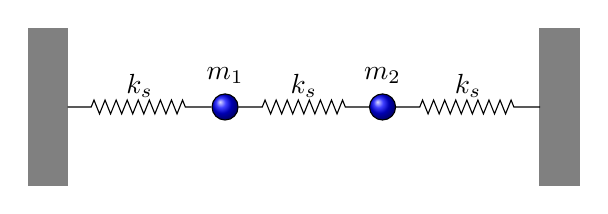
\begin{tikzpicture}
[wall/.style = {gray,fill=gray},
mass/.style = {draw,circle,ball color=blue},
spring/.style = {decorate,decoration={zigzag, pre length=.3cm,post length=.3cm,segment length=#1}},]
\draw[wall] (-.5,-1) rectangle (0,1);
\coordinate (l) at (0,0);
\node[mass,label={above:$m_1$}] (m1) at (2,0) {};
\node[mass,label={above:$m_2$}] (m2) at (4,0) {};
\coordinate (r) at (6,0);
\draw[wall] (6,-1) rectangle (6.5,1);

\draw[spring=4pt] (l) -- node[above] {$k_s$} (m1);
\draw[spring=4pt] (m1) -- node[above] {$k_s$} (m2);
\draw[spring=4pt] (m2) -- node[above] {$k_s$} (r);
\end{tikzpicture}  
\caption{\textit{The scenario of springs and masses in Exercise \ref{ex:hooke}.}}
\end{figure}
\end{Exercise}